
%DIF LATEXDIFF DIFFERENCE FILE
%DIF DEL head.tex                 Mon Feb 16 14:55:45 2015
%DIF ADD adhocnow15_bolster.tex   Mon Feb 16 12:08:09 2015
%%%%%%%%%%%%%%%%%%%%%%% file adhocnow15_bolster.tex %%%%%%%%%%%%%%%
%[Ad Hoc Now 2015](http://www.netmode.ntua.gr/adhocnow2015/index.html)
%
%# Dates
%* Deadline: 7/2/15
%* Acceptance: 7/3/15
%* Due: 28/3/15
%* Dates: 29/6/15-2/7/15
%
%# Topics of Interest
%* Access Control 
%* Ad Hoc Networks of Autonomous Intelligent Systems 
%* Algorithmic Issues
%* Analytic Methods and Modeling for Performance Evaluation 
%* Ad Hoc Network Applications and Architectures 
%* Delay-Tolerant Networking
%* Distributed Algorithms for Ad Hoc Networks 
%* Energy Efficiency 
%* Geometric Graphs
%* Location Discovery and Management 
%* Mobility Handling and Utilization 
%* Wireless Mesh Networks
%* Big Data Inspired Data Sensing
%* Mobile Ad Hoc Computing Platforms
%* Systems and Testbeds 
%* Mobile Social Networking 
%* Quality-of-Service 
%* Routing Protocols (Unicast, Multicast, etc.) 
%* Secure Services and Protocols 
%* Sensor Networks 
%* Self-Configuration 
%* Service Discovery 
%* Timing Synchronization 
%* Vehicular Networks 
%* Wireless Internet
%* Processing and Networking Technologies Complexity and Computational Issues
%* Prototype systems and real-world deployment experiences
%
%# Proposed Area of Focus
%Re-present Bellas Chap 4 work with extensions to explain and explore differences between Ad Hoc and Marine.
%
%
%%%%%%%%%%%%%%%%%%%%%%%%%%%%%%%%%%%%%%%%%%%%%%%%%%%%%%%%%%%%%%%%%%%


\documentclass[runningheads,a4paper]{llncs}

\usepackage{amssymb}
\usepackage{amsmath}
\setcounter{tocdepth}{3}
\usepackage{graphicx}
%DIF 53a53-61
\usepackage{float} %DIF > 
 %DIF > 
% Added to fix Table input %DIF > 
\usepackage{booktabs} %DIF > 
\usepackage{subcaption} %DIF > 
 %DIF > 
% Added to enhance todo lists, possibly need deleted pre pub %DIF > 
\usepackage{todonotes} %DIF > 
\usepackage{hyperref} %DIF > 
%DIF -------

\usepackage{url}
\newcommand{\keywords}[1]{\par\addvspace\baselineskip
\noindent\keywordname\enspace\ignorespaces#1}
%DIF PREAMBLE EXTENSION ADDED BY LATEXDIFF
%DIF UNDERLINE PREAMBLE %DIF PREAMBLE
\RequirePackage[normalem]{ulem} %DIF PREAMBLE
\RequirePackage{color}\definecolor{RED}{rgb}{1,0,0}\definecolor{BLUE}{rgb}{0,0,1} %DIF PREAMBLE
\providecommand{\DIFaddtex}[1]{{\protect\color{blue}\uwave{#1}}} %DIF PREAMBLE
\providecommand{\DIFdeltex}[1]{{\protect\color{red}\sout{#1}}}                      %DIF PREAMBLE
%DIF SAFE PREAMBLE %DIF PREAMBLE
\providecommand{\DIFaddbegin}{} %DIF PREAMBLE
\providecommand{\DIFaddend}{} %DIF PREAMBLE
\providecommand{\DIFdelbegin}{} %DIF PREAMBLE
\providecommand{\DIFdelend}{} %DIF PREAMBLE
%DIF FLOATSAFE PREAMBLE %DIF PREAMBLE
\providecommand{\DIFaddFL}[1]{\DIFadd{#1}} %DIF PREAMBLE
\providecommand{\DIFdelFL}[1]{\DIFdel{#1}} %DIF PREAMBLE
\providecommand{\DIFaddbeginFL}{} %DIF PREAMBLE
\providecommand{\DIFaddendFL}{} %DIF PREAMBLE
\providecommand{\DIFdelbeginFL}{} %DIF PREAMBLE
\providecommand{\DIFdelendFL}{} %DIF PREAMBLE
%DIF END PREAMBLE EXTENSION ADDED BY LATEXDIFF
%DIF PREAMBLE EXTENSION ADDED BY LATEXDIFF
%DIF HYPERREF PREAMBLE %DIF PREAMBLE
\providecommand{\DIFadd}[1]{\texorpdfstring{\DIFaddtex{#1}}{#1}} %DIF PREAMBLE
\providecommand{\DIFdel}[1]{\texorpdfstring{\DIFdeltex{#1}}{}} %DIF PREAMBLE
%DIF END PREAMBLE EXTENSION ADDED BY LATEXDIFF

\begin{document}

\mainmatter  % start of an individual contribution

% first the title is needed
\title{DRAFT: Trust Framework Operation in Autonomous Marine Communications Environments}
\DIFdelbegin %DIFDELCMD < \subtitle{In Preparation for Submission Ad-Hoc Now 2015, Athens, June 29 - July 02 2015. Deadline 07 Feb 2015}
%DIFDELCMD < %%%
\DIFdelend \DIFaddbegin \subtitle{In Preparation for Submission Ad-Hoc Now 2015, Athens, June 29 - July 02 2015. Deadline 20th Feb 2015}
\DIFaddend 

% a short form should be given in case it is too long for the running head
\titlerunning{Trust Framework Operation in Marine Communications Environments}

% the name(s) of the author(s) follow(s) next
%
% NB: Chinese authors should write their first names(s) in front of
% their surnames. This ensures that the names appear correctly in
% the running heads and the author index.
%
\author{Andrew Bolster%
\DIFdelbegin %DIFDELCMD < \thanks{Please note that the LNCS Editorial assumes that all authors have used
%DIFDELCMD < the western naming convention, with given names preceding surnames. This determines
%DIFDELCMD < the structure of the names in the running heads and the author index.}
%DIFDELCMD < %%%
\DIFdelend %DIF > \thanks{Please note that the LNCS Editorial assumes that all authors have used the western naming convention, with given names preceding surnames. This determines the structure of the names in the running heads and the author index.}
, Alan Marshall, Ji Guo}
%
\authorrunning{Trust Framework Operation in Marine Communications Environments}
% (feature abused for this document to repeat the title also on left hand pages)

% the affiliations are given next; don't give your e-mail address
% unless you accept that it will be published
\institute{Advanced Networks Research Group, \\Department of Electrical Engineering \& Electronics,\\
University of Liverpool, UK\\
\url{{andrew.bolster,alan.marshall}@liv.ac.uk}\\
\url{http://www.anrg.liv.ac.uk/}}

%DIF < %%%%%%%%%%%%%%%%%%%%%%%%%%%%%%%%%%%%%%%%%%%%%%%%%%%%%%%%%%%%%%%%%%%%%%%%%%%%%%%%%%%%%%%%%%%%%
\DIFdelbegin %DIFDELCMD < \toctitle{THIS IS JUST FOR KEEPING TRACK OF STRUCTURAL CHANGES IN THE DRAFT}
%DIFDELCMD < \tocauthor{IGNORE ME}
%DIFDELCMD < %%%
\DIFdelend \maketitle   
\DIFdelbegin %DIFDELCMD < \tableofcontents                                                 %%%
%DIF < DELETE ME BEFORE PUBLICATION
%DIF < %%%%%%%%%%%%%%%%%%%%%%%%%%%%%%%%%%%%%%%%%%%%%%%%%%%%%%%%%%%%%%%%%%%%%%%%%%%%%%%%%%%%%%%%%%%%%
%DIFDELCMD < 

%DIFDELCMD < %%%
%DIF < \maketitle                                                   %UNCOMMENT ME BEFORE PUBLICATION
%DIFDELCMD < 

%DIFDELCMD < %%%
%DIF < %%%%%%%%%%%%%%%%%%%%%%%%%%%%%%%%%%%%%%%%%%%%%%%%%%%%%%%%%%%%%%%%%%%%%%%%%%%%%%%%%%%%%%%%%%%%%
\DIFdelend 

\begin{abstract}
  This paper presents a Trust Management Framework (TMF) for Marine Autonomous Networks, 
  \DIFdelbegin \DIFdel{including a critique of previous group work in this area utilising Fuzzy Sets and Gray Theory.
  }\DIFdelend We present a comparative study on the operation and performance of such trust frameworks between \DIFdelbegin \DIFdel{the }\DIFdelend \DIFaddbegin \DIFadd{a typical }\DIFaddend terrestrial and the harsh underwater communications \DIFdelbegin \DIFdel{environments. 
  }\DIFdelend \DIFaddbegin \DIFadd{environment, examining the scaling factors involved (periodicity, physical spacing, etc.) in comparing and contrasting these environments.
}

  \DIFaddend We demonstrate the need for a different approach towards metric selection and trust-timing in such constrained networks.
  \keywords{ad-hoc, MANET, trust, marine, underwater, acoustic}
\end{abstract}

\section{Introduction}\label{sec:introduction}

As mobile ad-hoc networks (MANETs) grow beyond the terrestrial arena, their operation and the protocols designed around them must be reviewed to assess their suitability and optimality in different communications environments to ensure their continued security, reliability, and performance.

Trust Management Frameworks (TMFs) provide information to assist the estimation of future states and operations of nodes within networks.
This information is used to optimize the performance of a system of systems in the face of malicious, selfish, or defective \DIFdelbegin \DIFdel{behavior }\DIFdelend \DIFaddbegin \DIFadd{behaviour }\DIFaddend by one or more nodes within such a system.
Previous research has established the advantages of implementing distributed TMFs in terrestrial, 802.11 based mobile ad-hoc networks (MANETs), particularly in terms of preventing selfish operation in constrained collaborative systems \cite{Li2007}, and maintaining throughput in the presence of malicious actors \cite{Buchegger2002}

Current TMFs generally use a single type of observed action to derive trust metrics, i.e. successfully forwarded packets. These historical observations then inform future decisions of individual nodes, for example, the selection of a forward router with the lowest previous Packet Loss Rate (PLR) \cite{Li2008}.

Recent work has demonstrated \DIFdelbegin \DIFdel{the }\DIFdelend use of a number of metrics \DIFdelbegin \DIFdel{together, forming a �}\DIFdelend \DIFaddbegin \DIFadd{to form a '}\DIFaddend vector’ of trust.
In the case of \DIFaddbegin \DIFadd{Multi-parameter trust framework for MANETs (MTMF)}\DIFaddend \cite{Guo2012}, these metrics related to inter-node communications.
This vectorized trust allows a system to detect anomalous \DIFdelbegin \DIFdel{behavior }\DIFdelend \DIFaddbegin \DIFadd{behaviour }\DIFaddend and identify the tactics being used to undermine or subvert trust.

\DIFdelbegin \DIFdel{However, }\DIFdelend \DIFaddbegin \DIFadd{To date }\DIFaddend this work has been limited to terrestrial, RF based, communications networks.
As \DIFdelbegin \DIFdel{Autonomous }\DIFdelend \DIFaddbegin \DIFadd{autonomous }\DIFaddend underwater vehicles (AUVs) become more capable, and economical, they are being used in \DIFdelbegin \DIFdel{a }\DIFdelend many defence, commercial and environmental applications.
These applications are tending towards utilising  independent collective behaviour of teams or fleets of these platforms \cite{Caiti2011}
With this use being increasingly independent of classical command and control structures, the accurate and timely establishment of mutual and distributed communications trust between nodes within such fleets is essential for the reliability and stability of such systems, and to the secure integration of such systems into larger management systems-of-systems.
\DIFdelbegin %DIFDELCMD < 

%DIFDELCMD < %%%
\DIFdelend As such, the application of Trust methods developed in the \DIFdelbegin \DIFdel{Terrestrial }\DIFdelend \DIFaddbegin \DIFadd{terrestrial }\DIFaddend MANET space must be re-appraised for application within the challenging underwater communications channel.

\DIFdelbegin \subsection{\DIFdel{Paper Structure}}
%DIFAUXCMD
\addtocounter{subsection}{-1}%DIFAUXCMD
%DIFDELCMD < 

%DIFDELCMD < %%%
\DIFdel{In section }\DIFdelend \DIFaddbegin \DIFadd{The paper is laid out as follows.
In Section }\DIFaddend \ref{sec:trustandtmfs} we discuss Trust and Trust Management Frameworks, defining our terminology and reviewing the justifications for the use and development of Trust Management Frameworks.
\DIFdelbegin \DIFdel{We then review the results presented in \mbox{%DIFAUXCMD
\cite{Guo11}
}%DIFAUXCMD
and discuss the differences in experimental setup when transitioning to the marine space.
In section }\DIFdelend \DIFaddbegin \DIFadd{In Section }\DIFaddend \ref{sec:marineacousticnetworks}, we review selected features of the underwater communications channel, highlighting particular challenges and differentials against terrestrial equivalents.
In \DIFdelbegin \DIFdel{section \ref{sec:initialsystemcharacterisation}we }\DIFdelend \DIFaddbegin \DIFadd{Section \ref{sec:initialsystemcharacterisation}, we review the results presented in \mbox{%DIFAUXCMD
\cite{Guo11}
}%DIFAUXCMD
, including a critique of the use of Fuzzy Sets and Gray Theory and a discussion on differences in experimental configuration when transitioning from terrestrial radio to the marine space. 
We }\DIFaddend establish the initial parameters for simulation and set out a series of experiments to establish commonality between trust establishment in \DIFdelbegin \DIFdel{Terrestrial and Marine }\DIFdelend \DIFaddbegin \DIFadd{terrestrial and marine }\DIFaddend networks, characterising the communications and physical configuration with respect to the application and channel characteristics.
In \DIFdelbegin \DIFdel{section }\DIFdelend \DIFaddbegin \DIFadd{Section }\DIFaddend \ref{sec:trustresultsanddiscussion}, we present our findings in trust establishment in this optimal network, pointing out the differences in metric selection and their impact on trust assessment stability.

\DIFdelbegin \subsection{\DIFdel{Contributions}}
%DIFAUXCMD
\addtocounter{subsection}{-1}%DIFAUXCMD
\DIFdelend \DIFaddbegin \DIFadd{The contributions to the field of this paper are:
}\todo{Needs to be converted to prose}
\DIFaddend \begin{itemize}
  \item A Trust Management Framework applicable to Underwater MANETs \DIFaddbegin \DIFadd{and why Grey Theory Analysis is particularly suited to this application}\DIFaddend .
  \item A study on the \DIFdelbegin \DIFdel{comparitive }\DIFdelend \DIFaddbegin \DIFadd{comparative }\DIFaddend operation and performance between \DIFdelbegin \DIFdel{Terrestrial and Underwater }\DIFdelend \DIFaddbegin \DIFadd{terrestrial and underwater }\DIFaddend MANETs.
  \item A review of metric suitability for Trust Management Frameworks in \DIFdelbegin \DIFdel{Marine Environments}\DIFdelend \DIFaddbegin \DIFadd{marine environments}\DIFaddend , informing future metric selection for experimenters and theorists.
\end{itemize}

\section{Trust and Trust Management Frameworks}\label{sec:trustandtmfs}

\subsection{Trust in MANETs}\label{sec:trustinmanets}

In human trust relationships it \DIFdelbegin \DIFdel{can be seen }\DIFdelend \DIFaddbegin \DIFadd{is recognised }\DIFaddend that there can be several perspectives of Trust for example organizational, sociological, interpersonal, psychological and neurological \cite{Lee2004}.
\DIFdelbegin %DIFDELCMD < 

%DIFDELCMD < %%%
\DIFdelend For the purposes of this work we define two perspectives on trust for autonomous systems: Design and Operational. These are summarised as follows:

\begin{itemize}
  \item \emph{Design Trust}; When an autonomous system is under development a level of Trust is established in it through the manner in which it has been designed and tested.
    This is the same as conventional systems.
    The difference with systems that have high-levels of autonomy is that they are designed to behave adaptively to dynamic environments that are difficult to fully predict prior to operational deployment.
    For example, in a navigation system it is difficult to predict the dynamic environment it will need to adapt to.
    So Trust needs to be developed that the design and test of such systems are sufficient to predict that operation will be, if not optimal, at least satisfactory.

  \item \emph{Operational Trust}; Trust at runtime or in-situ that both the individual nodes within a system are operating as expected\footnote{Operational Trust is functionally derived from, but distinct from Design Trust}; and that the interfaces between the operator and the system are as expected.
    This latter aspect covers issues such as physical/wireless links and interpretation of data at each end of such a communication link.
\end{itemize}

In addition to the two perspectives of trust identified, it is necessary to define and classify Operational Trust into two distinct but related sections, which we define as being:
\begin{itemize}
  \item \emph{Hard Trust} or technical trust, being the quantitative measurement and communication of the expectation of an actor performing a certain task, based on historic performance and through consensus building within a networked system.
    Can be thought of as a de-risking strategy to measure and monitor the ability of a system, or another actor within a system, to perform a task unsupervised.
  \item \emph{Soft Trust} or common trust, being the qualitative assessment of the ability of an actor to perform a task or operation consistently and reliably based on social or experiential factors.
    This is the ‘natural’ form of trust and is the main motivational driver for the human-factors trust discussion.
    Can be rephrased as the level of confidence an operator has in an actor to perform a task unsupervised.
\end{itemize} 

% THIS COULD COME IN HANDY LATER % It is already clear that these two definitions are extremely close in their construction, but represent fundamentally different approaches to trust, one coming from a sociological perspective of person-to-person and person-to-group relationships from day to day life, and the other coming from a statistical or formal appraisal of an activity by a system.
For the purposes of this work, we are concerned with the analytical establishment of hard trust within a topologically dynamic network of autonomous actors.

\subsection{Current Trust Management Frameworks}

Various models and algorithms for describing trust and developing trust management in distributed systems, P2P communities or wireless networks have been considered.
Taking \DIFdelbegin \DIFdel{two }\DIFdelend \DIFaddbegin \DIFadd{some }\DIFaddend examples;

\begin{itemize}
  \item \emph{The Objective Trust Management Framework} takes a Bayesian \DIFdelbegin \DIFdel{network }\DIFdelend approach and introduces the idea of applying a Beta function to changes in the per-link Packet Loss Rate (PLR) over time as an encapsulation method, combining ``Trust'' and ``Confidence of Assessment'' into a single value \cite{Li2008}.
    OTMF however does not appropriately combat multi-node-collusion in the network \cite{Cho2011}.

  \item \emph{Trust-based Secure Routing \cite{Moe2008a}} demonstrated an extension to Dynamic Source Routing (DSR), incorporating a Hidden Markov Model of the wider ad-hoc network, reducing the efficacy of Byzantine attacks, particularly black-hole attacks but, along with many more TMFs surveyed in \cite{Cho2011}, falls under the same limitation of focusing on single metric observation (PLR).
  \item \emph{CONFIDANCE}; \DIFdelbegin \textbf{\DIFdel{DRAFT: Add \mbox{%DIFAUXCMD
\cite{Buchegger2002}
}%DIFAUXCMD
in here if there's space, or find something more recent built on it}}
%DIFAUXCMD
\DIFdelend \DIFaddbegin \DIFadd{\mbox{%DIFAUXCMD
\cite{Buchegger2002}
}%DIFAUXCMD
presented an approach using a probabilistic estimation of normal observations, generating a posterior probability distribution of node forwarding behaviours, similar to OTMF. They also introduced a greedy topology weighting scheme that internally weighted incoming trust assessments based on historical experience of the reporter.
}\DIFaddend \end{itemize}

These \DIFaddbegin \DIFadd{approaches can be generalised as single-value probabilistic estimation, based around a Bayesian idea of taking a binary input state and generating an idealised Beta Distribution (\ref{eq:beta}) of the future states of that input generated through an expectation value based on interactions (\ref{eq:beta_e}).
}

\begin{align}\DIFadd{
  \label{eq:beta}
  \text{beta}(p|\alpha,\beta) = \frac{\Gamma(\alpha + \beta)}{\Gamma(\alpha)\Gamma(\beta)}p^{\alpha-1},\text{ where } 0 \leq p \leq 1; \alpha,\beta > 0}\\
  \DIFadd{\label{eq:beta_e}
  E(p) = \frac{\alpha}{\alpha + \beta}
}\end{align}

\DIFadd{Where $\alpha$ and $\beta$ represent the number of successful and unsuccessful interactions respectively.
}

\DIFadd{These }\DIFaddend single metric TMFs provide malicious actors with a significant advantage if their activity is undetectable by that one assessed metric, especially if the attacker knows the metric in advance.

\DIFaddbegin \DIFadd{There are situations where the observed metrics will include significant noise involved with complicated interdependencies between the environment and the system under observation; and those observations themselves occur at irregular, sparse, intervals.
In such cases, conventional approaches such as Bayesian prior probability estimation do not produce trust values that fairly reflect the underlying metrics, as they require a-prioi assumption that the trust value under exploration has a known or expected distribution (Beta), that that distribution is monomodal, and that the input metrics are binary discernible.
These assumptions are required to scale and classify resultant trust values to a stable assessment range (usually $[0,1]$) \mbox{%DIFAUXCMD
\cite{Liu2006}
}%DIFAUXCMD
.
In scenarios with variable, sparse, noisy metrics, estimating the distribution is difficult to accomplish off-line in advance.
Further, the binary requirement of Bayesian-style modelling requires internal discriminating logic, which discards useful information from a multi-node perspective, and generating a phase transition area where a proportion of negative or malicious behaviour does not impact the assessed trust observations of other nodes, but still impacts system performance \mbox{%DIFAUXCMD
\cite{Mundinger2008}
}%DIFAUXCMD
. 
}

\DIFadd{Finally, there is no accounting for the context in which the assessment is taking place; while OTMF does include topological information, it does not take account of environmental factors that may be inducing poor performance.
}

\begin{table}[h]
  \caption{\DIFaddFL{Comparison between selected methods of characterising uncertainty, adapted from \mbox{%DIFAUXCMD
\cite{Ng1994}
}%DIFAUXCMD
\mbox{%DIFAUXCMD
\cite{Liu2006}
}%DIFAUXCMD
\mbox{%DIFAUXCMD
\cite{Wang2006}
}%DIFAUXCMD
\mbox{%DIFAUXCMD
\cite{Guo11}
}%DIFAUXCMD
}}
  \label{tab:uncertainty}
  \begin{center}
    \setlength{\tabcolsep}{8pt}
    \begin{tabular}{l|ccc}
      \toprule
        & \DIFaddFL{Fuzzy Math }& \DIFaddFL{Probabilistic Estimation }& \DIFaddFL{Grey Systems }\\
      \midrule
      \DIFaddFL{Objects }& \DIFaddFL{Cognitive Uncertainty }& \DIFaddFL{Distribution Refinement }& \DIFaddFL{Poor Information }\\
      \DIFaddFL{Set Style }& \DIFaddFL{Fuzzy Sets }& \DIFaddFL{Cantor Sets }& \DIFaddFL{Grey Hazy Sets }\\
      \DIFaddFL{Methodology }& \DIFaddFL{Discerning Affiliation }& \DIFaddFL{Probability Distribution }& \DIFaddFL{Information Coverage }\\
      \DIFaddFL{Processes }& \DIFaddFL{Marginal Sampling }& \DIFaddFL{Frequency Distribution }& \DIFaddFL{Sequence Generation }\\
      \DIFaddFL{Data Requirement }& \DIFaddFL{Known Membership }& \DIFaddFL{Beta Distribution }& \DIFaddFL{Any Distribution }\\
      \DIFaddFL{Emphasis }& \DIFaddFL{Extension }& \DIFaddFL{Intension }& \DIFaddFL{Intension }\\
      \DIFaddFL{Objective }& \DIFaddFL{Cognitive Expression }& \DIFaddFL{Stabilisation }& \DIFaddFL{Realism }\\
      \DIFaddFL{Characteristics }& \DIFaddFL{Experience }& \DIFaddFL{Large Samples }& \DIFaddFL{Small Samples}\\
     \bottomrule
    \end{tabular}
    \setlength{\tabcolsep}{6pt}
  \end{center}
\end{table}


\DIFadd{Grey Theory counters this by performing cohort based normalisation of metrics at runtime. 
This creates a more stable contextual assessment of trust, providing an ``extent'' of potential trust values with respect to other observed nodes in that interval rather, while still maintaining the ability to reduce trust values down to a stable assessment range for decision support without having to characterise every environment entered into.}\footnote{\DIFadd{A potential negative to this approach is that since the assessment is relative in nature (as opposed to the absolutist approach to trust assumed in other frameworks), even in ideal operating networks, nodes will receive middling trust assessments, as there is no-one else ``bad'' to compete against. Future work will investigate the stability of GRA under multi-node collusion}}

\DIFaddend The objective of operating a TMF is to increase the confidence in, and efficiency of, a system by reducing the amount of undetectable negative operations an attacker can perform.
This \DIFdelbegin \DIFdel{space }\DIFdelend \DIFaddbegin \DIFadd{``set'' }\DIFaddend of potential attacks can be described as \DIFdelbegin \DIFdel{the ‘Threat Surface�}\DIFdelend \DIFaddbegin \DIFadd{a ``threat surface''}\DIFaddend .
In the case where the attacker can subvert the TMF, the metric under assessment by that TMF does not cover the threat mounted by the attacker.
In turn, this causes a super-linearly negative effect in the efficiency of the network as the TMF is assumed to have reduced the threat surface when in fact it has only made it more advantageous to attack a \DIFdelbegin \DIFdel{facet }\DIFdelend \DIFaddbegin \DIFadd{different aspect }\DIFaddend of the networks operation.
\DIFdelbegin \DIFdel{\mbox{%DIFAUXCMD
\cite{Huang2010a}
}%DIFAUXCMD
also raised the need for a more expanded view of trust but did so with a domain-partitioning approach rather than combining trust assessments from multiple domains within networks}\DIFdelend \DIFaddbegin \DIFadd{An example of such a behaviour would be the case in a TMF focused on PLR where an attacker selectively delays packets going through it, reducing the over all throughput of one or more virtual network routes.
Such behaviour would not be detected by the TMF}\DIFaddend .

\DIFaddbegin \todo{Need to lead from single metric assessment to multi-metric}\DIFaddend \subsection{Grey Relational Trust for Terrestrial MANETs}

\cite{Guo2012} demonstrated the ability of Grey Relational Analysis (GRA)\cite{Zuo1995} to normalize and operationally combine disparate traits of a communications link such as instantaneous throughput, received signal strength, etc. into a single comparable value, a Grey Relational Coefficient, or a ``trust vector''.
\DIFdelbegin \DIFdel{This vector is given
}\DIFdelend \DIFaddbegin 

\DIFadd{In the case of the terrestrial communications network used in \mbox{%DIFAUXCMD
\cite{Guo2012}
}%DIFAUXCMD
, the observed metric set $X = \{x_1,\dots,x_M\}$ representing the measurements taken by each node of its neighbours at least interval, is defined as 
}\begin{equation}\DIFadd{
  \label{eq:terrmetrics}
  X=\{\text{packet loss rate, signal strength, data rate, delay, throughput}\}
}\end{equation}

\DIFadd{The trust vector is then given as
}\DIFaddend 

\begin{align}
  \label{eq:grc}
  \theta_{k,j}^t = \frac{\min_k|a_{k,j}^t - g_j^t| + \rho \max_k|a_{k,j}^t-g_j^t|}{|a_{k,j}^t-g_j^t| + \rho \max_k|a_{k,j}^t-g_j^t|} \\
  \phi_{k,j}^t = \frac{\min_k|a_{k,j}^t - b_j^t| + \rho \max_k|a_{k,j}^t-b_j^t|}{|a_{k,j}^t-b_j^t| + \rho \max_k|a_{k,j}^t-b_j^t|}  \DIFaddbegin \\
  [\DIFadd{\theta_k^t, \phi_k^t}] \DIFadd{= }[\DIFadd{(\theta_{k,0}^t,}\dots\DIFadd{,\theta_{k,M}^t),(\phi_{k,0}^t,}\dots\DIFadd{,\phi_{k,M}^t )}]
\DIFaddend \end{align}

where $a_{k,j}^t$ is the value of a observed metric \DIFdelbegin \DIFdel{$j$ }\DIFdelend \DIFaddbegin \DIFadd{$x_j$ }\DIFaddend for a given node $k$ at time $t$, $\rho$ is a distinguishing coefficient normally set to $0.5$, $g$ and $b$ are respectively the 'good' and 'bad' reference metric sequences from $\{a_{k,j}^t, k=1,2\dots K\}$, e.g. $g_j=\max_k({a_{k,j}^t})$,  $b_j=\min_k({a_{k,j}^t})$ (where each metric is selected to be monotonically increasingly positive for trust assessment, \DIFdelbegin \DIFdel{eg Throughput}\DIFdelend \DIFaddbegin \DIFadd{e.g. throughput}\DIFaddend ). $\theta$ and $\phi$ are then scaled to $[0,1]$ using the mapping $y = 1.5 x - 0.5$.
The vector natures of \DIFdelbegin \DIFdel{$[\theta,\phi]$ }\DIFdelend \DIFaddbegin \DIFadd{$[\theta_k^t,\phi_k^t]$ }\DIFaddend allow per-metric weighting before generating a single trust assessment, and also allows the identification and classification of untrustworthy agents.
These weighted $[\theta,\phi]$ values are then condensed into a single trust value by
\begin{equation}
  \label{eq:trustvalue}
  T_k^t = \frac{1}{1+\frac{(\phi_k^t)^2}{(\theta_k^t)^2}}
\end{equation}
\DIFdelbegin \DIFdel{For applications involving low fidelity, temporally sparse metrics with unknown statistical distributions, GRA is a more stable comparative analysis, providing an interval of potential trust values rather than fuzzy-logic or the Bayesian-Beta distributions found in current TMFs \mbox{%DIFAUXCMD
\cite{Liu2006}
}%DIFAUXCMD
. 
}\DIFdelend 

GRA, combined with a fuzzy whiteization model \eqref{eq:whitenization}, and a topology-aware weighting scheme\eqref{eq:networkeffects} \DIFaddbegin \footnote{\DIFadd{similar to that employed in CONFIDANT}} \DIFaddend provide capability to both detect the existence of a malicious agent within the network, and to classify what trust metrics that attacker is manipulating\DIFdelbegin \DIFdel{, identifying the style of attack taking place}\DIFdelend .

There are three classes of topological trust relationship; Direct, Recommendation, and Indirect.
To take the example of a node $n_i$ monitoring the trust of another, target, node, $n_j$; the Direct relationship is simply the trust assessment based on $n_i$'s own observations and experience of $n_j$'s behaviour.
In the Recommendation case, another node, $n_k$, which shares direct relationships with both $n_i$ and $n_j$, gives it's opinion on the trustworthiness of $n_j$ to $n_i$.
The Indirect case is similar to the recommendation case, except that the recommender $n_k$, does not have a (current) direct link with the target $n_j$ but that has a direct link with the observer node, $n_i$.

These relationships give us node sets, $N_R$ and $N_I$ containing the nodes that have recommendation or indirect, relationships to the observing node respectively.

\begin{align}
  \label{eq:whitenization}
  f_1(x) &= -x+1\notag\\
  f_2(x) &= 
  \begin{cases}
    2x & \text{if }x\leq 0.5\\
    -2x+2 & \text{if }x>0.5
  \end{cases}\\
  f_3(x) &= x\notag
\end{align}

\begin{align}
  \label{eq:networkeffects}
  T_{i,j}^{net}=&\frac{1}{2} \cdot \max_s\{f_s(T_{i,j})\} T_{i,j}&\qquad \text{Direct Trust}\notag \\
  &+ \frac{|N_R| }{2|N_R| + |N_I|}\sum_{n \in N_R} \max_s\{f_s(T_{i,n})\} T_{i,n}&\qquad \text{Recommendation Trust}\notag\\
  &+ \frac{|N_I| }{2|N_R| + |N_I|}\sum_{n \in N_I} \max_s\{f_s(T_{i,n})\} T_{i,n} &\qquad \text{Indirect Trust}
\end{align}

\DIFdelbegin \DIFdel{\mbox{%DIFAUXCMD
\cite{Guo11}
}%DIFAUXCMD
demonstrated the stochastic variation of this methodology wrt. attack method, enabling the detection and identification of the aspect of network operation under attack.
It is this work that is being expanded upon in paper.
}%DIFDELCMD < 

%DIFDELCMD < %%%
\DIFdelend \subsection{Scenarios}\DIFaddbegin \todo{Maybe move to Section \ref{sec:initialsystemcharacterisation}}
\DIFaddend 

Four Mobility scenarios were used in \cite{Guo11} to explore the trust-behaviour, covering the majority of MANET operational requirements; 

\begin{itemize}
  \item All Nodes Static
  \item Central node performing a random walk with leaf-nodes static
  \item Leaf-nodes randomly walking with central node static
  \item All nodes randomly walking
\end{itemize}

The six nodes \DIFdelbegin \DIFdel{were arranged in the form of a flattened pentagon with the 'central' node ($n_1$) placed near the geometric middle}\DIFdelend \DIFaddbegin \DIFadd{are arranged as per Fig. \ref{fig:s1_layout}}\DIFaddend , such that each node \DIFdelbegin \DIFdel{was }\DIFdelend \DIFaddbegin \DIFadd{is }\DIFaddend on average 100m from its neighbours. 
\DIFaddbegin \DIFadd{The use of six nodes and the particular layout enables the investigation of the three trust relationships based on minimum path topologies, such that the node generating the trust assessments, $n_0$ has Direct, Recommendation, and Indirect trust assessments available to it from itself, $[n_2,n_3]$, and $[n_4,n_5]$ respectively.
}\DIFaddend 

In all of the scenarios, each link from $n_i \rightarrow n_j$ sent \DIFdelbegin \DIFdel{a }\DIFdelend 10 second \DIFaddbegin \DIFadd{bursts }\DIFaddend of Constant Bit Rate (CBR) style traffic.

\begin{figure}[h]
  \centering
  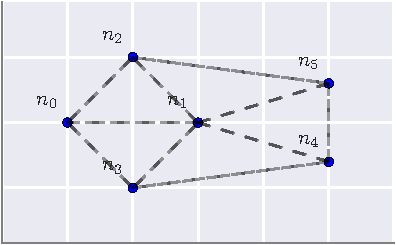
\includegraphics[width=0.45\textwidth]{img/s1_layout.pdf}
  \caption{Initial Scenario Topology, with nodes spaced an average of 100m apart}
  \label{fig:s1_layout}
\end{figure}

\DIFaddbegin \DIFadd{Guo demonstrated that when compared against OTMF and Beta trust assessment, MTFM provided increased variation in trust assessment over time, providing more information about the nodes behaviour than simply the probabilistic nature of packet delivery. Guo also demonstrated that this MTFM valuation was stochastically stable for varying mobilities. 
}


\DIFaddend \section{Marine Acoustic Networks}\label{sec:marineacousticnetworks}

The key challenges of underwater acoustic communications are centred around the impact of slow and differential propagation of energy (RF, Optical, Acoustic) through water, and it's interfaces with the seabed / air.
The resultant challenges include; long delays due to propagation, significant inter-symbol interference and Doppler spreading, fast and slow fading due to environmental effects (aquatic flora/fauna; surface weather), carrier-frequency dependent signal attenuation, multipath caused by the medium interfaces at the surface and seabed, variations in propagation speed due to depth dependant effects (salinity, temperature, pressure, gaseous concentrations and bubbling), and subsequent refractive spreading and lensing due to that same propagation variation\DIFdelbegin \DIFdel{.\mbox{%DIFAUXCMD
\cite{Partan2006}
}%DIFAUXCMD
}\DIFdelend \DIFaddbegin \DIFadd{\mbox{%DIFAUXCMD
\cite{Partan2006}
}%DIFAUXCMD
.
}\DIFaddend 

The attenuation that occurs in an underwater acoustic channel over a distance $d$ for a signal about frequency $f$ in linear and $dB$ forms respectively is given by

\begin{equation}
  \label{eq:acoattenuation}
  A(d,f) = A_0d^ka(f)^d
\end{equation}
\begin{equation}
  \label{eq:acoattenuationdb}
  10 \log A(d,f)/A_0 = k \cdot 10 \log d + d \cdot 10 \log a(f)
\end{equation}

where $A_0$ is a unit-normalising constant, $k$ is a spreading factor (commonly taken as 1.5), and $a(f)$ is the absorption coefficient, expressed empirically using Thorp's formula \eqref{eq:thorp} from \cite{Stojanovic2007}

\begin{equation}
  \label{eq:thorp}
  10 \log a(f) = 0.11 \cdot \frac{f^2}{1+f^2} + 44\cdot\frac{f^2}{4100+f^2}+ 2.75\times10^{-4} f^2 + 0.003
\end{equation}


Thus, the multi-path channel transfer function can be described by 

\begin{equation}
  \label{eq:acomultipath}
  H(d,f) =\sum_{p=0}^{P-1} h(p) = \sum_{p=0}^{P-1} \Gamma_p / \sqrt{A(d_p,f)}e^{-j 2 \pi f \tau_p}
\end{equation}

where $d=d_0$ is the minimal path length between the transmitter and receiver, $d_p,p=\{1,\dots P-1\}$ are the secondary path lengths, $\Gamma_p$ models additional losses incurred on each path such as reflection losses at the surface interface, and $\tau_p = d_p/c$ is the delay time ($c = 1500 ms^{-1}$ is the nominal speed of sound underwater).


This combination of refractive lensing and the multipath nature of the medium result in supposedly ``line of sight'' propagation being extremely unreliable for estimating distances to targets, as the first arriving beam has as the very least bent in the medium, and commonly has bounced between the surface/seabed before arriving at a receiver.
Further, this affect is usually anisotropic with differential depths between transmitter and receiver, meaning that any variation in depth across a channel, greatly impacts the characteristics of that channel.

Comparing \eqref{eq:acoattenuation} with the RF Free-Space Path Loss model \eqref{eq:fspl}, while both are frequency and distance dependant; 

\begin{equation}
  \label{eq:fspl}
  A_{rf}(d,f) \approx \left( \frac{4\pi f}{c} \right)^2
  \text{where }c\approx 3\times10^8m/s
\end{equation}



\subsection{Trust \DIFdelbegin \DIFdel{Requirement }\DIFdelend in Marine Networks}

\DIFaddbegin \todo{Justify Why Grey, discuss current uses and demand. Relate back to Section \ref{sec:trustinmanets}}\DIFaddend In this subsection we establish the requirement for communications trust in acoustic marine networks, extending and expanding on the generic assessment given in \ref{sec:trustinmanets}


\section{Initial System Model Characterisation}\label{sec:initialsystemcharacterisation}

\subsection{Simulation Background}

Simulations were conducted using a Python based agent simulation framework based on SimPy\cite{Mueller2003SimPy}, with a network stack built upon the AUVNetSim stack\cite{Miquel2008}, with transmission parameters \DIFaddbegin \DIFadd{(Table \ref{tab:sysconstraints}) }\DIFaddend taken from and validated against \cite{Stojanovic2007} and \cite{Stefanov2011}.

Given the differences in delay and propagation between RF and marine networks, it is natural that the same application rates (e.g. packet emission rates or throughput) cannot be \DIFdelbegin \DIFdel{maintained under such different constraints}\DIFdelend \DIFaddbegin \DIFadd{equal}\DIFaddend .
Therefore, before we can fairly assess the trust operation of a Underwater MANET, we first establish \DIFdelbegin \DIFdel{it's operational characteristics}\DIFdelend \DIFaddbegin \DIFadd{an equally operational zone of performance}\DIFaddend .

\DIFdelbegin \DIFdel{Specifically, we sought to }\DIFdelend \DIFaddbegin \DIFadd{We }\DIFaddend define a methodology for establishing \DIFdelbegin \DIFdel{a near-optimal operationpoint.
This was }\DIFdelend \DIFaddbegin \DIFadd{an comparative operating point in the marine environment that can account for the differences in communications environment while maintaining a comparable trust operation.
This is }\DIFaddend done in two parts; optimisation for \DIFdelbegin \DIFdel{network level queuing}\DIFdelend \DIFaddbegin \DIFadd{Communications Rate}\DIFaddend , optimisation for \DIFdelbegin \DIFdel{physical layout scaling}\DIFdelend \DIFaddbegin \DIFadd{Physical Distribution}\DIFaddend .

\DIFdelbegin %DIFDELCMD < \begin{table}[H]
%DIFDELCMD <   %%%
\DIFdelend \DIFaddbegin \begin{table}[h]
  \DIFaddendFL \caption{Comparison of system model constraints as applied between Terrestrial and Marine communications} \label{tab:sysconstraints}
  \begin{center}
    \setlength{\tabcolsep}{8pt}
    \DIFdelbeginFL %DIFDELCMD < \begin{tabular}{|l|c|c|c|}
%DIFDELCMD <       \hline
%DIFDELCMD <       %%%
\DIFdelendFL \DIFaddbeginFL \begin{tabular}{lccc}
      \toprule
      \DIFaddendFL Parameter & Unit & Terrestrial & Marine \\
      \DIFdelbeginFL %DIFDELCMD < \hline
%DIFDELCMD <       %%%
\DIFdelendFL \DIFaddbeginFL \midrule
      \DIFaddendFL Simulated Duration & $s$ & 300 & 36000\\
      Simulated Area & $km^2$ & 0.7 & \DIFdelbeginFL \DIFdelFL{0.7 }\DIFdelendFL \DIFaddbeginFL \DIFaddFL{Various }\DIFaddendFL \\
      Transmission Range & $km$ & 0.25 & 1.5 \\
      Number of Nodes & & 6 & 6 \\
      \DIFdelbeginFL \DIFdelFL{Comms Medium }\DIFdelendFL \DIFaddbeginFL \DIFaddFL{Physical Layer }\DIFaddendFL & & RF(802.11) & Acoustic\\
      Propagation Speed& $m/s$ & $3\times10^8$ & 1490\\
      Center Frequency& $Hz$ & $2.6\times10^9$ & \DIFdelbeginFL \DIFdelFL{$10^3$ }\DIFdelendFL \DIFaddbeginFL \DIFaddFL{$2 \times 10^3$ }\DIFaddendFL \\
      Bandwidth& $Hz$ & $22\times10^6$ & $10^3$\\
      MAC Type & & CSMA/CA & CSMA/CA\\
      Routing Protocol & & DSDV & FBR \\
      Mobility & & Various & Various \\
      Max Speed & $ms^{-1}$ & 5 & \DIFdelbeginFL \DIFdelFL{1.25 }\DIFdelendFL \DIFaddbeginFL \DIFaddFL{2.4 }\DIFaddendFL \\
      Data Rate & $bps$ & $10^6$ & 240 \\
      Burst Counts & & 10 & 1 \\
      Packet Size & bits & 4096 &  9600 \\
      Destination Selection & & Random & Random\\
      Single Transmission Duration & $s$ & 10 & 32 \\
      Single Transmission Size & bits & $10^7$ & $9600$ \\
      \DIFdelbeginFL %DIFDELCMD < \hline
%DIFDELCMD <     %%%
\DIFdelendFL \DIFaddbeginFL \bottomrule
    \DIFaddendFL \end{tabular}
    \setlength{\tabcolsep}{6pt}
  \end{center}
\end{table}


\subsection{Establishing Scale Factors in Communications Rate}

In this section we characterise the simulated communications environment, establishing an optimal packet emission rate for comparison against \cite{Guo11}.

In order to establish \DIFdelbegin \DIFdel{this 'saturation point '}\DIFdelend \DIFaddbegin \DIFadd{the point at which the network becomes saturated due}\DIFaddend , a range of packet emission rates were explored between 0.01 packets per second (pps), equivalent to 96 bps, up to 0.07 pps (672 bps)

From \DIFdelbegin \DIFdel{\ref{fig:throughput_performance_static} and }\DIFdelend \DIFaddbegin \DIFadd{Figs.~\ref{fig:throughput_performance_static} and ~}\DIFaddend \ref{fig:prod_breakdown_static}, it is clear that the threshold curve, expressed as the \emph{Successfully Received Packets} line, exhibits a saturation point between 0.025 and 0.03 \DIFdelbegin \DIFdel{bps}\DIFdelend \DIFaddbegin \DIFadd{pps}\DIFaddend .
Particularly in \DIFaddbegin \DIFadd{Fig.~}\DIFaddend \ref{fig:prod_breakdown_static}, the precipitous drop in packet delivery probability beyond 0.025 pps, indicating that this \DIFdelbegin \DIFdel{would be a safe operational zone }\DIFdelend \DIFaddbegin \DIFadd{is a strong candidate value for an upper-limit to the safe operating zone in terms of packet emission in the small static case}\DIFaddend .

\DIFdelbegin %DIFDELCMD < \begin{figure}[th!]
%DIFDELCMD <   %%%
\DIFdelend \DIFaddbegin \begin{figure}[H]
  \DIFaddendFL \centering
  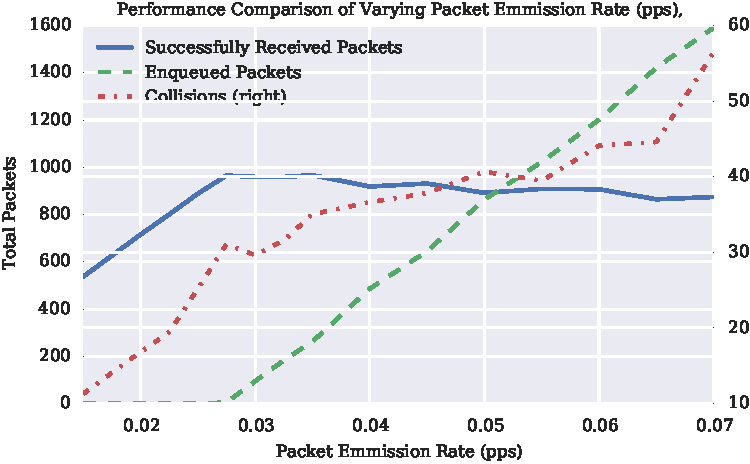
\includegraphics[width=0.6\textwidth]{img/throughput_performance_static.pdf}
  \caption{Varying packet emission rate demonstrates maximal throughput at 0.025 packets per second, equivalent to $\approx$240 bps}
  \label{fig:throughput_performance_static}
\end{figure}


\DIFdelbegin %DIFDELCMD < \begin{figure}[h!]
%DIFDELCMD <   %%%
\DIFdelend \DIFaddbegin \begin{figure}[H]
  \DIFaddendFL \centering
  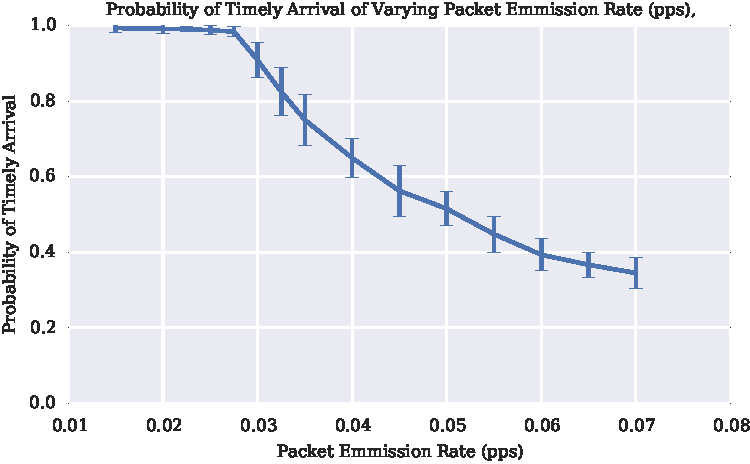
\includegraphics[width=0.6\textwidth]{img/prod_breakdown_static.pdf}
  \caption{Varying packet emission rate demonstrates a saturation point at 0.025 packets per second}
  \label{fig:prod_breakdown_static}
\end{figure}


\subsection{Establishing Scale Factors in Physical Distribution}

In this section we characterise the \DIFdelbegin \DIFdel{simulated communications environment, establishing an optimal }\DIFdelend \DIFaddbegin \DIFadd{effect of }\DIFaddend node-separation scaling \DIFaddbegin \DIFadd{on communications operation }\DIFaddend for comparison against \cite{Guo11}\DIFdelbegin %DIFDELCMD < 

%DIFDELCMD < %%%
\DIFdel{This is pretty much summarised in and \ref{fig:prod_breakdown_range} 
}\DIFdelend \DIFaddbegin \DIFadd{. This is particularly important considering the significant scale factor differences between not only the speed of propagation in the medium, but simply the range of operation. 
From Table \ref{tab:sysconstraints}, the operating transmission range of acoustic is $\approx 6$ times further than 802.11, indicating that a suitable operating environment will have an area $\approx \sqrt{6}$ times the area of the 802.11 case. Therefore, a reasonable experimental range would have an upper bound of performance around this scaling factor, where nodes are approximately 400$m$ apart. 
}

\DIFadd{A reasonable range around this is to scale from 100$m$ apart on average to 800$m$.
}

\DIFaddend Varying average node separation shows that while direct throughput isn't significantly affected until, collision rates are \DIFdelbegin \DIFdel{\ref{fig:throughput_performance_range}. However, this }\DIFdelend \DIFaddbegin \DIFadd{Fig.~\ref{fig:throughput_performance_range}.
This }\DIFaddend collision rate is well within the tolerances of the MAC layer, as shown in \DIFdelbegin \DIFdel{\ref{fig:prod_breakdown_range}}\DIFdelend \DIFaddbegin \DIFadd{Fig.~\ref{fig:prod_breakdown_range}, where even with a rising collision rate, packets are being reliably received}\DIFaddend .

\DIFdelbegin %DIFDELCMD < \begin{figure}[th!]
%DIFDELCMD <   %%%
\DIFdelend \DIFaddbegin \begin{figure}[H]
  \DIFaddendFL \centering
  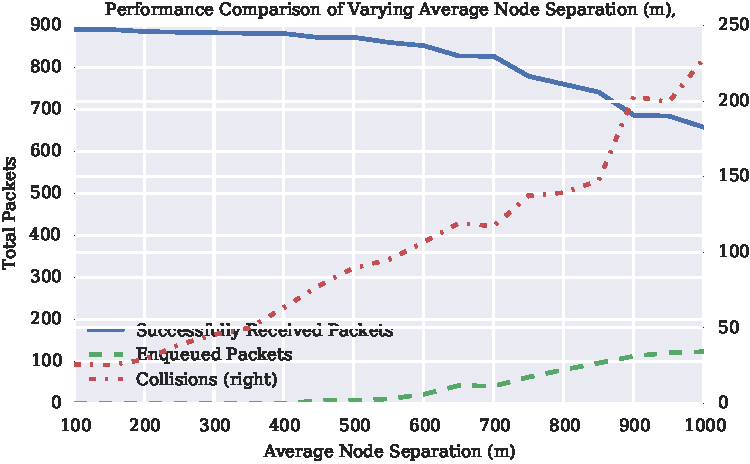
\includegraphics[width=0.6\textwidth]{img/throughput_performance_range.pdf}
  \caption{Comparison of Medium \DIFdelbeginFL \DIFdelFL{Access }\DIFdelendFL \DIFaddbeginFL \DIFaddFL{Acquisition }\DIFaddendFL Collisions, Throughput, and Enqueued packets against varying application packet emission rates.\DIFdelbeginFL \DIFdelFL{Scaling ratio of 3 indicated that the average distance between nodes has been tripled.}\DIFdelendFL }
  \label{fig:throughput_performance_range}
\end{figure}

\DIFdelbegin %DIFDELCMD < \begin{figure}[h!]
%DIFDELCMD <   %%%
\DIFdelend \DIFaddbegin \begin{figure}[H]
  \DIFaddendFL \centering
  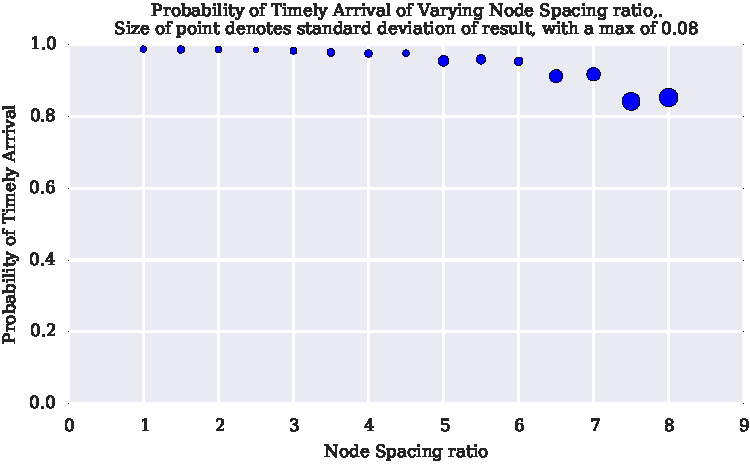
\includegraphics[width=0.6\textwidth]{img/prod_breakdown_range.pdf}
  \caption{\DIFdelbeginFL \DIFdelFL{Graph of probability }\DIFdelendFL \DIFaddbeginFL \DIFaddFL{Probability }\DIFaddendFL of \DIFdelbeginFL \DIFdelFL{timely reception }\DIFdelendFL \DIFaddbeginFL \DIFaddFL{Timely Reception }\DIFaddendFL across a range of node scaling.}
  \label{fig:prod_breakdown_range}
\end{figure}

\DIFdelbegin %DIFDELCMD < \begin{figure}[h!]
%DIFDELCMD <   %%%
\DIFdelend \DIFaddbegin \DIFadd{However, when end-to-end delay is investigated, it's clear from Fig.~\ref{fig:delay_range} that the network is becoming severely impaired approaching the 600$m$ mark, with delays rising to more than 25 minutes above 700$m$.
This is also demonstrated by the increasing RTS/Data ratio shown in Fig.~\ref{fig:rts_range}.
}

\DIFadd{According to Xu \mbox{%DIFAUXCMD
\cite{Xu2002}
}%DIFAUXCMD
, the RTS/CTS handshake cannot function well as interference protection at node separations beyond 0.56 times the transmission range. 
This is also demonstrated in  Fig.~\ref{fig:rts_range}, where above $1500m \times 0.56 = 840m$, 
This is due to reduced channel availability due to collisions, which are then due to a much longer potential contention period between nodes. 
}

\begin{figure}[H]
  \DIFaddendFL \centering
  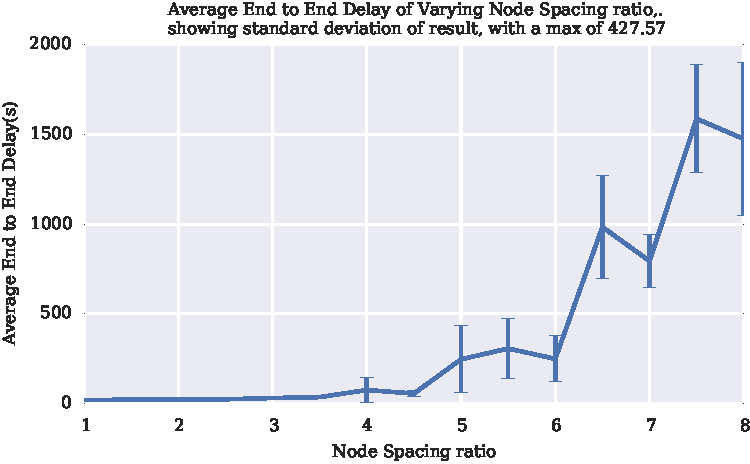
\includegraphics[width=0.6\textwidth]{img/delay_range.pdf}
  \caption{\DIFdelbeginFL \DIFdelFL{Varying average node separation shows that while direct throughput isn't affected, collision rates are. However, this collision rate is well within the tolerances of the MAC layer}\DIFdelendFL \DIFaddbeginFL \DIFaddFL{End to End Delay under varying node-separations}\DIFaddendFL }
  \label{fig:delay_range}
\end{figure}

\DIFdelbegin \subsubsection*{\DIFdel{Acknowledgments.}} %DIFAUXCMD
\DIFdel{The heading should be treated as a
subsubsection heading and should not be assigned a number}\DIFdelend \DIFaddbegin \begin{figure}[H]
  \centering
  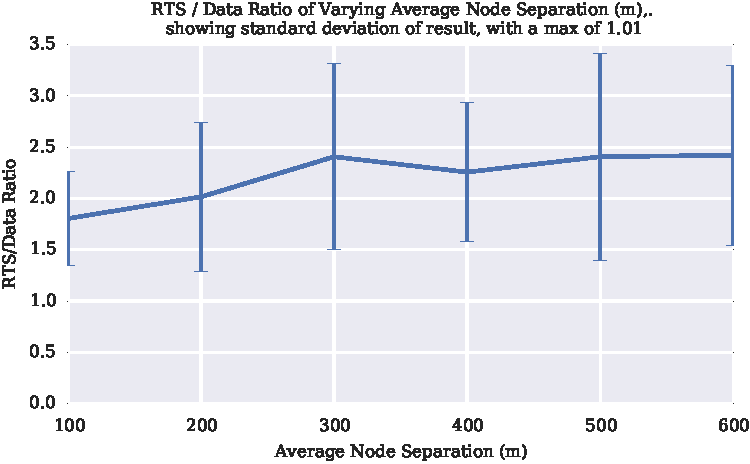
\includegraphics[width=0.6\textwidth]{img/rts_range.pdf}
  \caption{\DIFaddFL{RTS/Data ratio for varying node-separations}}
  \label{fig:rts_range}
\end{figure}


\begin{table}[H]
  \caption{\DIFaddFL{Tabular view of data from Figs~\ref{fig:prod_breakdown_range}, \ref{fig:delay_range}, and \ref{fig:rts_range}}} \label{tab:rangedelay}
  \begin{center}
      \hyphenpenalty \DIFaddFL{100000
      }\begin{tabular}{
*{2}{@{\hspace{1em}}r@{\hspace{1em}}}
*{3}{@{\hspace{1em}}p{0.1\textwidth} @{\hspace{1em}}}  }
\toprule
 Separation(m) &  Delay(s) &  Probability of Arrival &  RTS/Data Ratio &  Ideal Delivery Time(s) \\
\midrule
           100 &     60.32 &                    0.99 &            1.80 &                    1.03 \\
           200 &    419.95 &                    0.97 &            2.02 &                    1.10 \\
           300 &   1205.66 &                    0.89 &            2.41 &                    1.17 \\
           400 &   1288.20 &                    0.91 &            2.26 &                    1.25 \\
           500 &   1868.20 &                    0.87 &            2.41 &                    1.32 \\
           600 &   2191.07 &                    0.85 &            2.42 &                    1.39 \\
\bottomrule
\end{tabular}

  \end{center}
\end{table}

\subsection{\DIFadd{Scaling Discussion}}

\DIFadd{We establish a appropriate safe operating zone for marine communications by looking at the communications rate and physical distribution factors together as a 3D surface.
We select throughput and end to end delay as the targeted aspects of the networks performance to optimise against.
The raw results of these two metrics in the static scenario are shown in Fig.~\ref{fig:2d_delay_throughput}.
We take the ratio of throughput per second of delay as a combined proxy for this optimisation. $T/d$
}

\DIFadd{Fig.~\ref{fig:2d_ratio_static} demonstrates that there is a severe drop off in performance in stable performance in increasing packet emission rates above 0.02, even though Fig.~\ref{fig:2d_delay_static} on it's own would indicate an optimal zone in at a much higher rate.
However, due to increased medium contention and queueing delays at these rates enter into the order of hours, which is unacceptable for many applications.
These results indicate that the best area to continue operating in for a variety of node separations is at 0.015pps, and that a reasonable position scaling is from 100m to 600m, beyond which communication becomes increasingly unstable, especially in terms of end to end delay.
}

\begin{figure}
\begin{subfigure}{.5\textwidth}
  \centering
  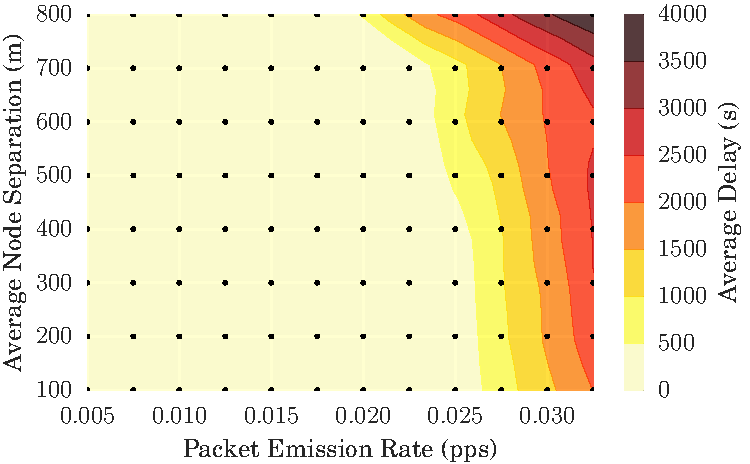
\includegraphics[width=.8\linewidth]{img/delay_2d_static.pdf}
  \caption{\DIFaddFL{Average Packet Delay (seconds)}}
  \label{fig:2d_delay_static}
\end{subfigure}%DIF > 
\begin{subfigure}{.5\textwidth}
  \centering
  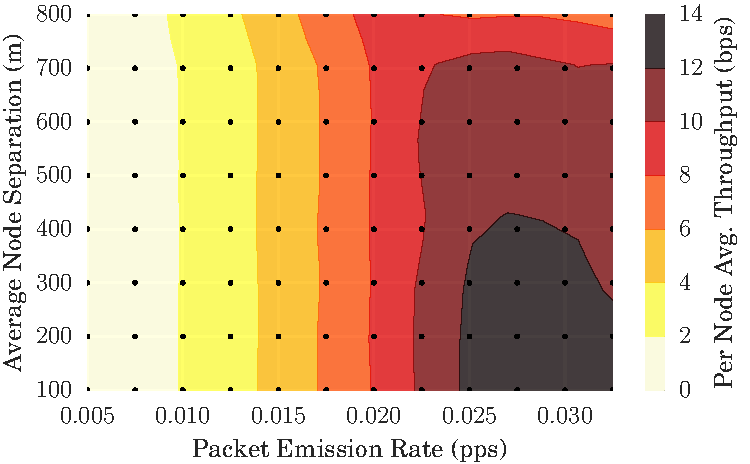
\includegraphics[width=.8\linewidth]{img/throughput_2d_static.pdf}
  \caption{\DIFaddFL{Throughput (packets)}}
  \label{fig:2d_throughput_static}
\end{subfigure}
\begin{subfigure}{.5\textwidth}
\centering
  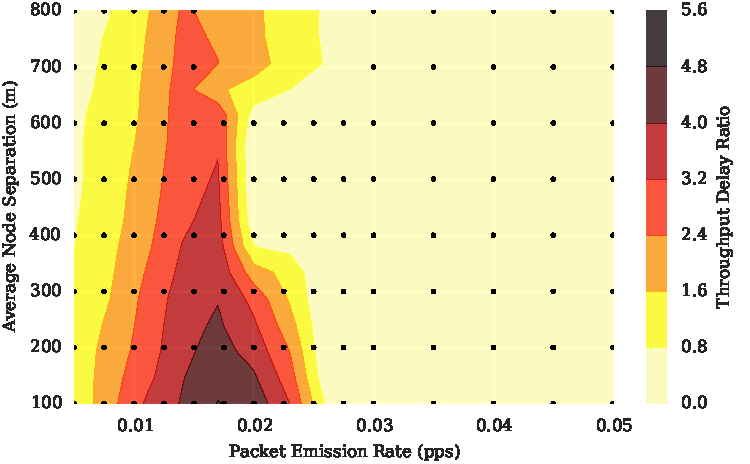
\includegraphics[width=.8\linewidth]{img/2d_ratio_static.pdf}
  \caption{\DIFaddFL{Throughput Delay Ratio}}
  \label{fig:2d_ratio_static}
\end{subfigure}
\begin{subfigure}{.5\textwidth}
\centering
  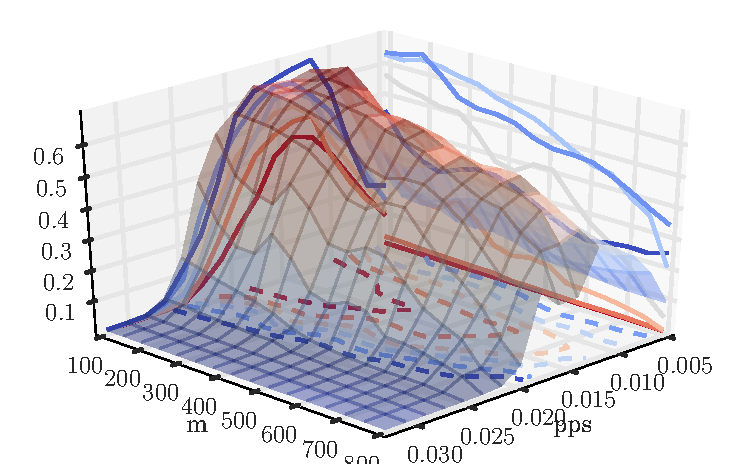
\includegraphics[width=.8\linewidth]{img/3d_ratio_static.pdf}
  \caption{\DIFaddFL{Normalised Surface Plot}}
  \label{fig:3d_ratio_static}
\end{subfigure}
\caption{\DIFaddFL{Field of Results for Varying Packet Emission Rates and Node Separations.}}
\label{fig:2d_delay_throughput_static}
\end{figure}\todo{could possibly lose everything but the TP/D R}

\section{\DIFadd{Trust}}\label{sec:trustresultsanddiscussion}

\DIFadd{Having established a safe operating range for comparison, we proceed to repeat the scenarios presented in \mbox{%DIFAUXCMD
\cite{Guo11}
}%DIFAUXCMD
in this simulated marine network.
}

\DIFadd{The particular factors under discussion are the relative performance of MTMF against OTMF and Beta with respect to statistical stability across scenarios and in responsiveness to changing network behaviour. 
We establish a similar result set by initially tracking the resultant trust values established by MTMF in each of the four mobility scenarios.
For simplicity, we are primarily concerned with the observational trust relationship between node 0 and node 1, i.e. $n_0$'s assessment of the trustworthiness of $n_1$, or $T_{1,0}$.
We are also concerned with the opinions of $n_1$ provided to $n_0$ by other nodes, where ${T_{1,2},T_{1,2}$ and ${T_{1,2},T_{1,2}$ denote the sets of recommendation and indirect trust assessments respectively.
Also included are a set of aggregate assessments; $T_{1,\text{avg}}$, the flat average of direct trust assessments of $n_1$, $T_{1,\text{Net}}$, an aggregate that weights assessments according to the network topology from }\eqref{eq:networkeffects}\DIFadd{, and $T_{1,\text{MTMF}}$, the final MTMF trust assessment value based on both network topology and whitenisation from }\eqref{eq:whitenization}\DIFadd{.
}


\DIFadd{From Fig.~\ref{fig:trust_static}, the generated trust values utilising the topology information ($T_{1,\text{Net}},T_{1,\text{MTMF}}$) display a greatly decreased variation than those of the individual subjective observations.
}

\begin{figure}
\begin{subfigure}{.5\textwidth}
  \centering
  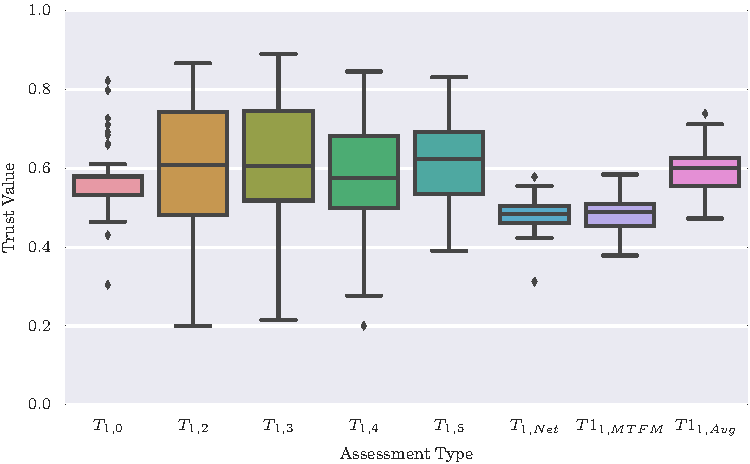
\includegraphics[width=.8\linewidth]{img/trust_bella_static.pdf}
  \caption{\DIFaddFL{All Nodes Static}}
  \label{fig:trust_static}
\end{subfigure}%DIF > 
\begin{subfigure}{.5\textwidth}
  \centering
  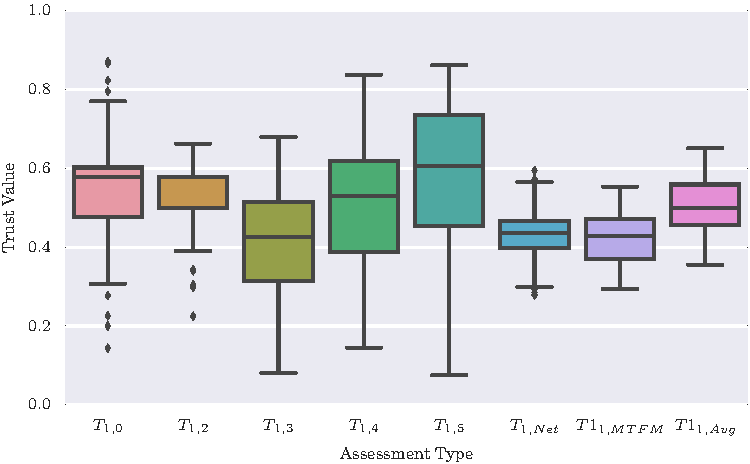
\includegraphics[width=.8\linewidth]{img/trust_bella_single_mobile.pdf}
  \caption{\DIFaddFL{$n_1$ Randomly Walking}}
  \label{fig:trust_single}
\end{subfigure}
\begin{subfigure}{.5\textwidth}
\centering
  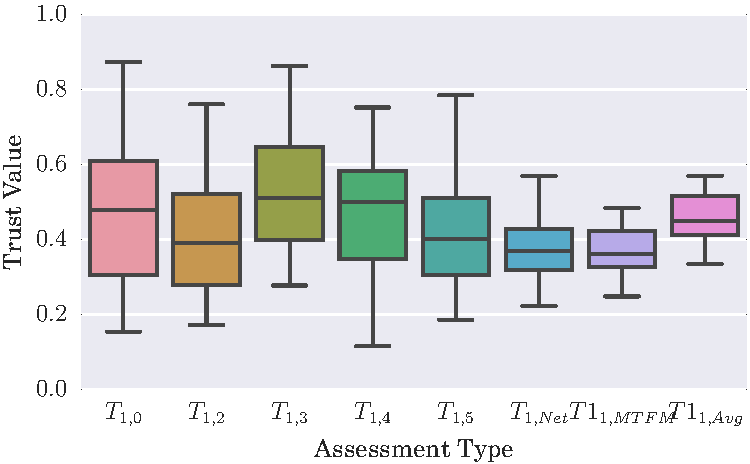
\includegraphics[width=.8\linewidth]{img/trust_bella_allbut1_mobile.pdf}
  \caption{\DIFaddFL{All Nodes but $n_1$ Randomly Walking}}
  \label{fig:trust_allbut1}
\end{subfigure}
\begin{subfigure}{.5\textwidth}
\centering
  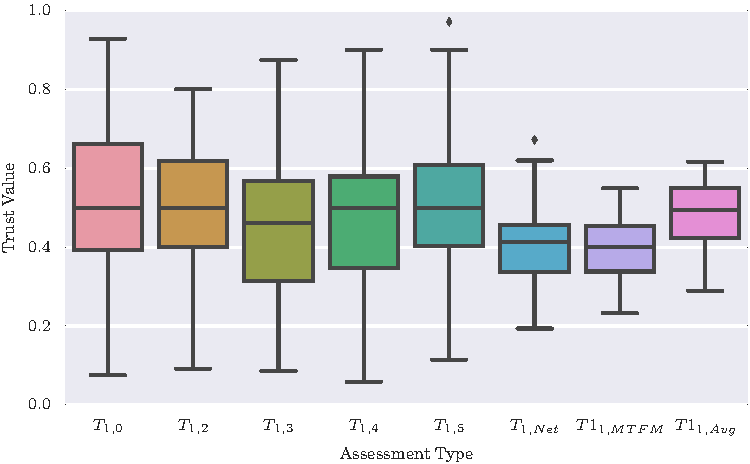
\includegraphics[width=.8\linewidth]{img/trust_bella_all_mobile.pdf}
  \caption{\DIFaddFL{All Nodes Randomly Walking}}
  \label{fig:trust_all_mobile}
\end{subfigure}
\caption{\DIFaddFL{MTMF Trust assessments for varying mobility options}}
\label{fig:trust_mobility}
\end{figure}

\begin{figure}
\begin{subfigure}{.5\textwidth}
  \centering
  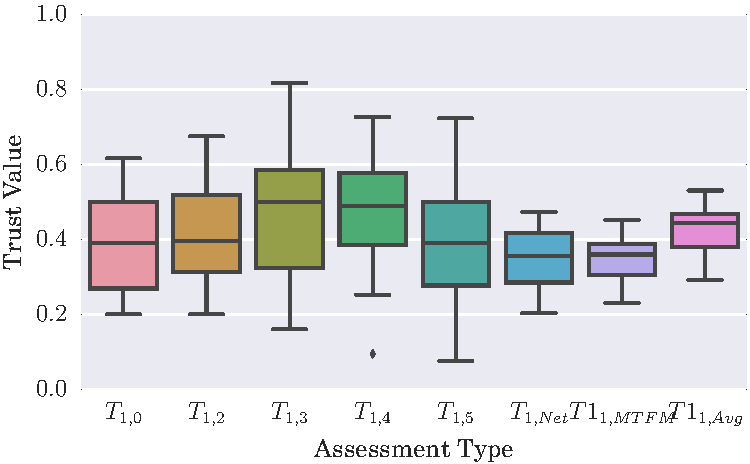
\includegraphics[width=.8\linewidth]{img/trust_bella_static_selfish.pdf}
  \caption{\DIFaddFL{All Nodes Static}}
  \label{fig:trust_static}
\end{subfigure}%DIF > 
\begin{subfigure}{.5\textwidth}
  \centering
  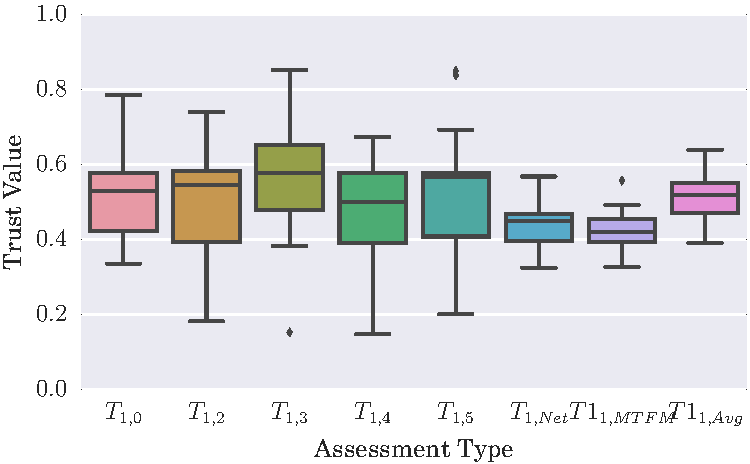
\includegraphics[width=.8\linewidth]{img/trust_bella_single_mobile_selfish.pdf}
  \caption{\DIFaddFL{$n_1$ Randomly Walking}}
  \label{fig:trust_single}
\end{subfigure}
\begin{subfigure}{.5\textwidth}
\centering
  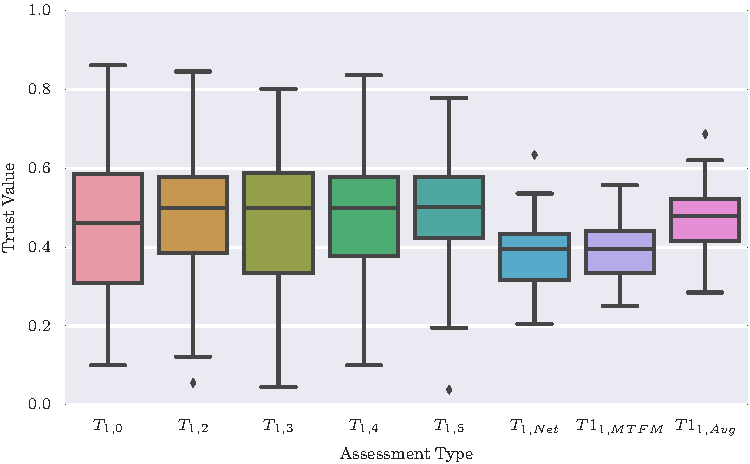
\includegraphics[width=.8\linewidth]{img/trust_bella_allbut1_mobile_selfish.pdf}
  \caption{\DIFaddFL{All Nodes but $n_1$ Randomly Walking}}
  \label{fig:trust_allbut1}
\end{subfigure}
\begin{subfigure}{.5\textwidth}
\centering
  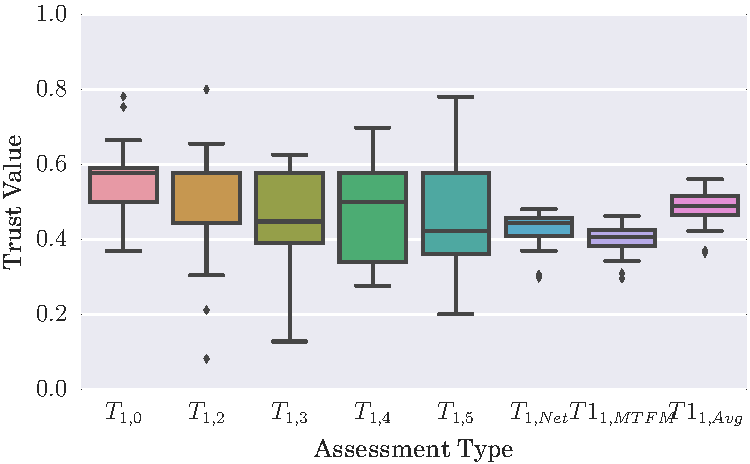
\includegraphics[width=.8\linewidth]{img/trust_bella_all_mobile_selfish.pdf}
  \caption{\DIFaddFL{All Nodes Randomly Walking}}
  \label{fig:trust_all_mobile}
\end{subfigure}
\caption{\DIFaddFL{MTMF Trust assessments for varying mobility options}}
\label{fig:trust_mobility}
\end{figure}

\begin{figure}
\begin{subfigure}{\textwidth}
  \centering
  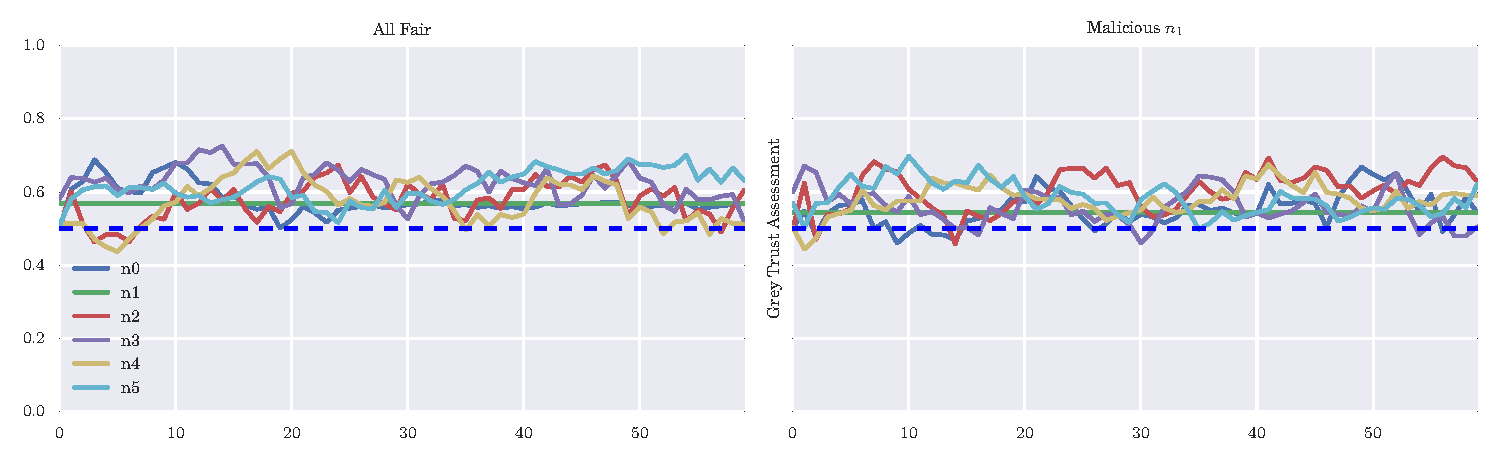
\includegraphics[width=.8\linewidth]{img/grey_trust_bella_static_joint.pdf}
  \caption{\DIFaddFL{All Nodes Static}}
  \label{fig:grey_trust_static}
\end{subfigure}
\begin{subfigure}{\textwidth}
  \centering
  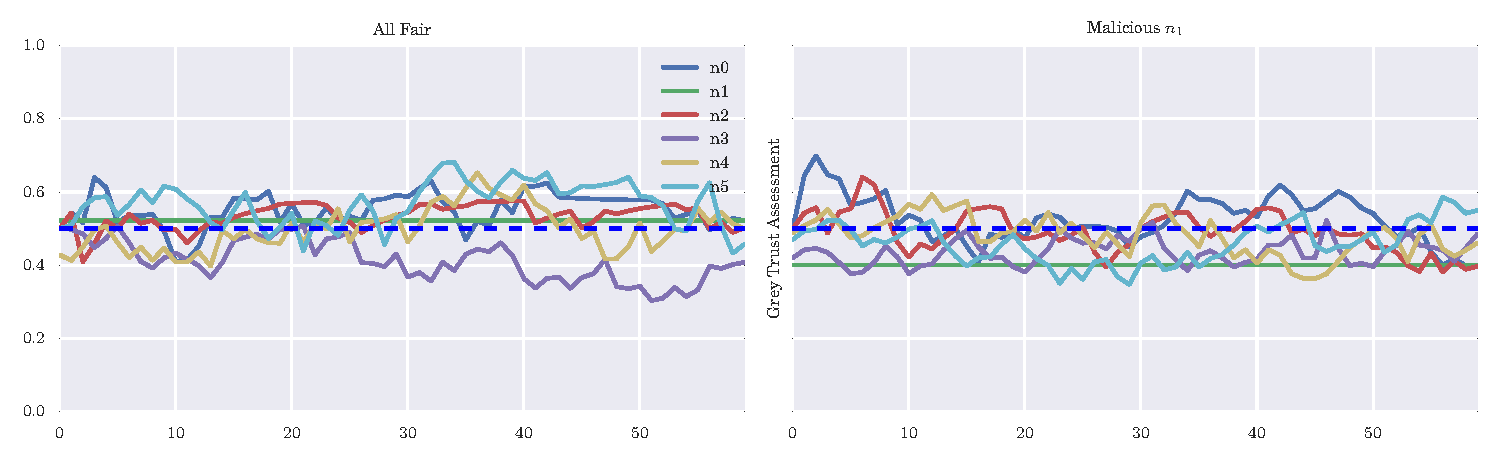
\includegraphics[width=.8\linewidth]{img/grey_trust_bella_single_mobile_joint.pdf}
  \caption{\DIFaddFL{$n_1$ Randomly Walking}}
  \label{fig:grey_trust_single}
\end{subfigure}
\begin{subfigure}{\textwidth}
\centering
  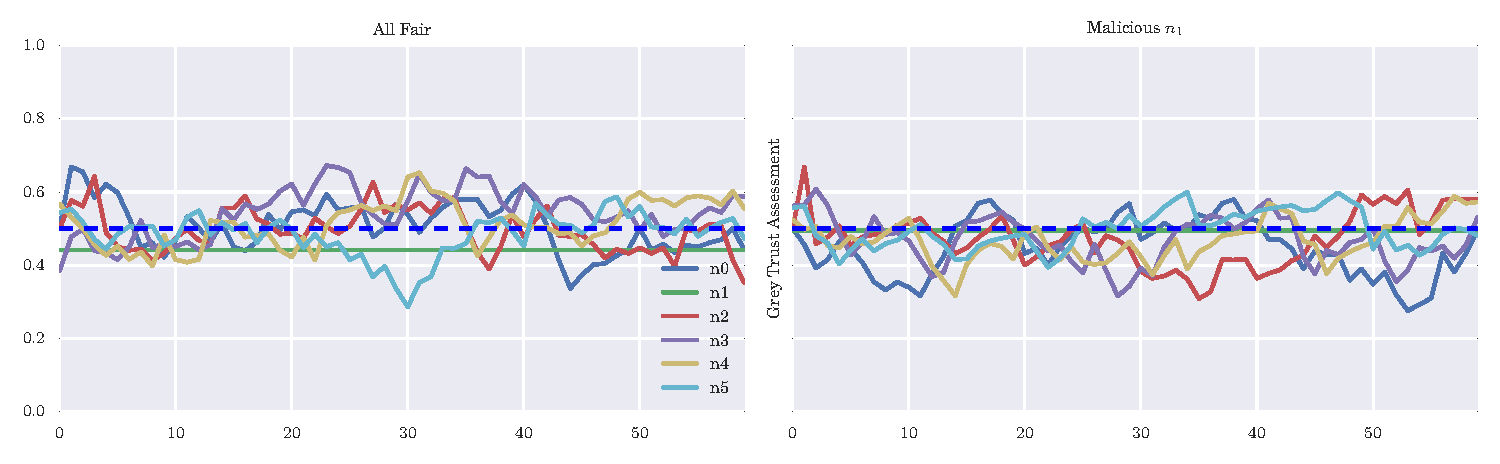
\includegraphics[width=.8\linewidth]{img/grey_trust_bella_allbut1_mobile_joint.pdf}
  \caption{\DIFaddFL{All Nodes but $n_1$ Randomly Walking}}
  \label{fig:grey_trust_allbut1}
\end{subfigure}
\begin{subfigure}{\textwidth}
\centering
  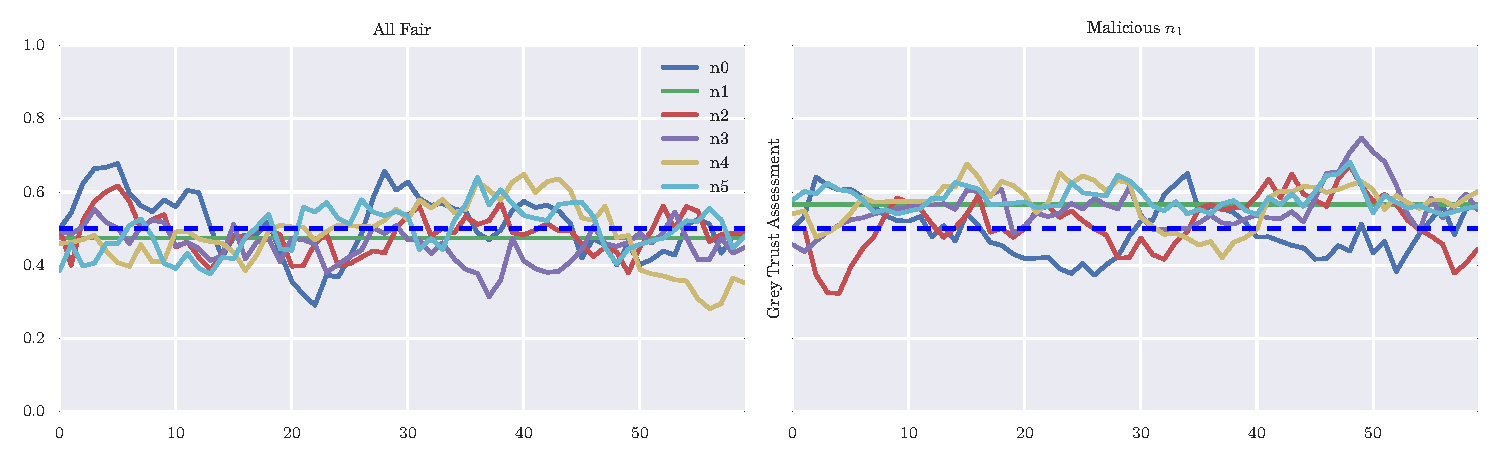
\includegraphics[width=.8\linewidth]{img/grey_trust_bella_all_mobile_joint.pdf}
  \caption{\DIFaddFL{All Nodes Randomly Walking}}
  \label{fig:grey_trust_all_mobile}
\end{subfigure}
\caption{\DIFaddFL{MTMF Trust time varying assessments for of $n1$ varying mobility options}}
\label{fig:trust_mobility}
\end{figure}

\begin{figure}
\begin{subfigure}{\textwidth}
  \centering
  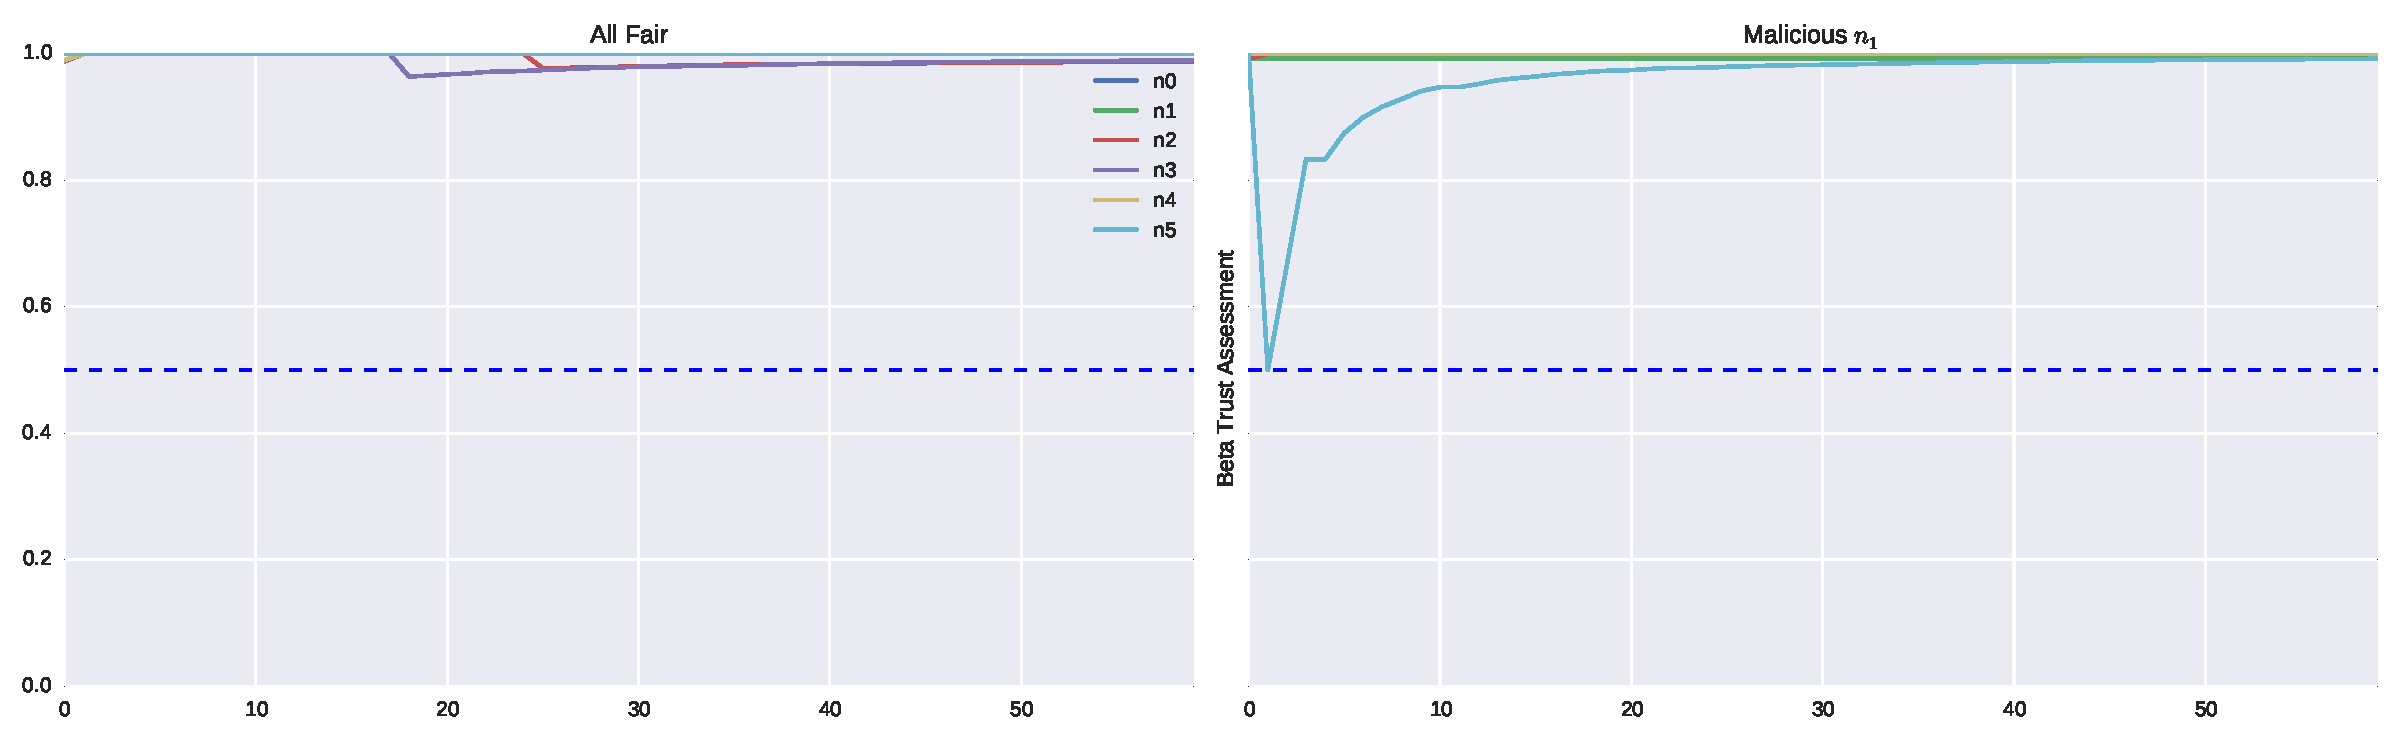
\includegraphics[width=.8\linewidth]{img/beta_trust_bella_static_joint.pdf}
  \caption{\DIFaddFL{All Nodes Static}}
  \label{fig:beta_trust_static}
\end{subfigure}
\begin{subfigure}{\textwidth}
  \centering
  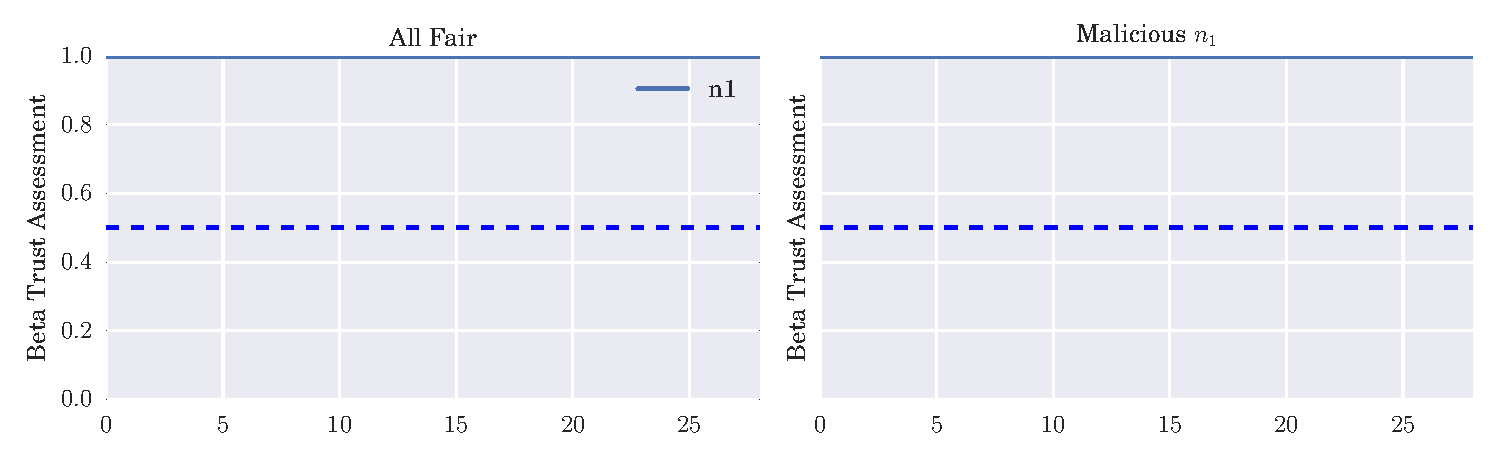
\includegraphics[width=.8\linewidth]{img/beta_trust_bella_single_mobile_joint.pdf}
  \caption{\DIFaddFL{$n_1$ Randomly Walking}}
  \label{fig:beta_trust_single}
\end{subfigure}
\begin{subfigure}{\textwidth}
\centering
  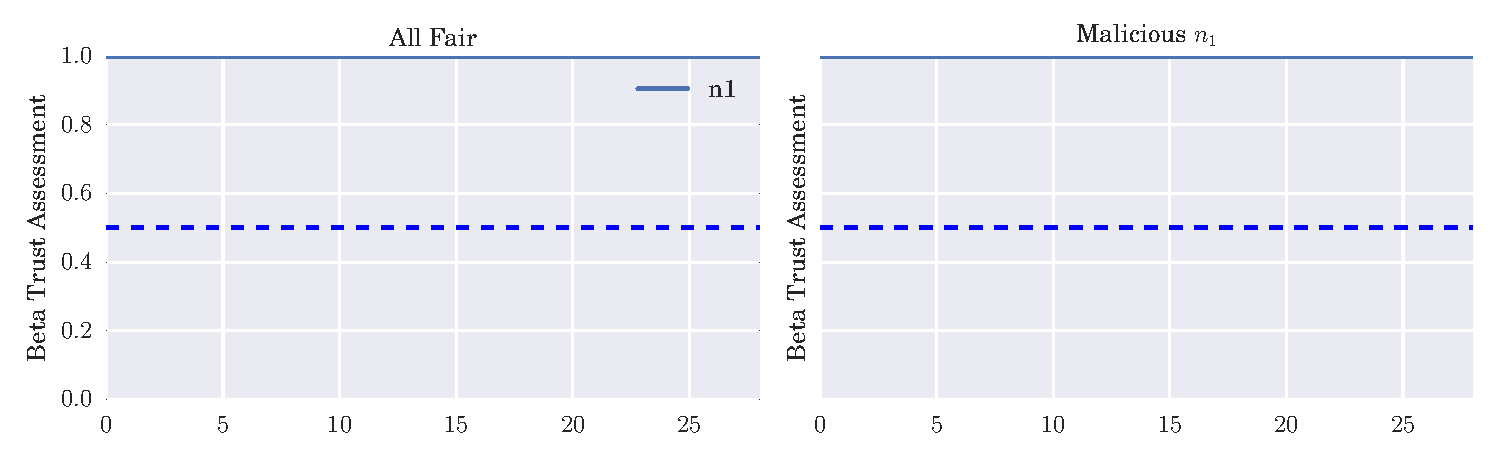
\includegraphics[width=.8\linewidth]{img/beta_trust_bella_allbut1_mobile_joint.pdf}
  \caption{\DIFaddFL{All Nodes but $n_1$ Randomly Walking}}
  \label{fig:beta_trust_allbut1}
\end{subfigure}
\begin{subfigure}{\textwidth}
\centering
  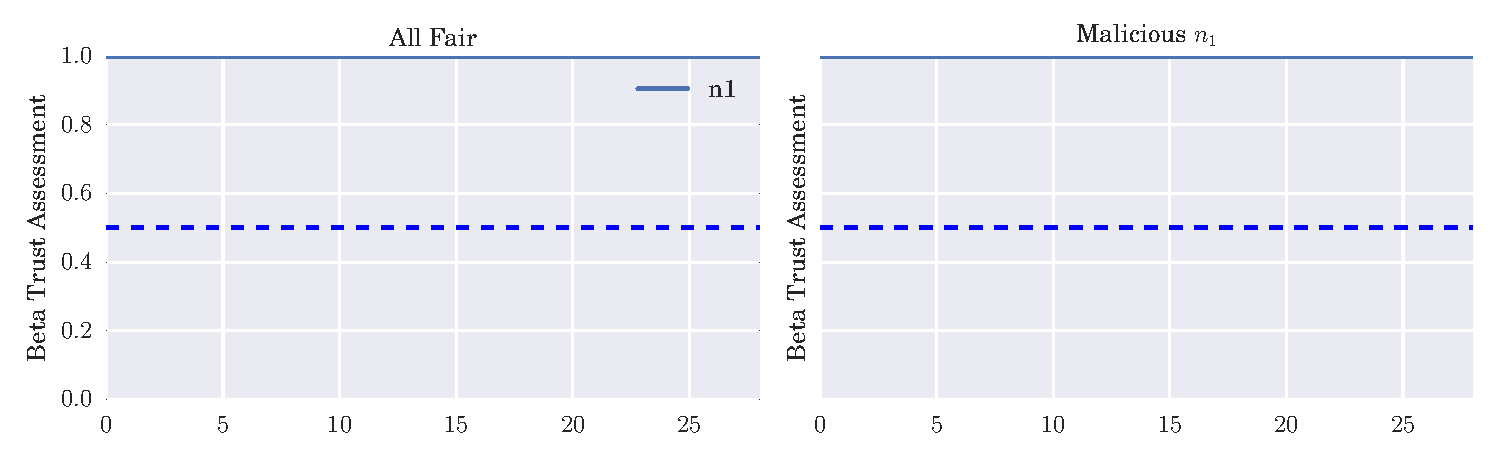
\includegraphics[width=.8\linewidth]{img/beta_trust_bella_all_mobile_joint.pdf}
  \caption{\DIFaddFL{All Nodes Randomly Walking}}
  \label{fig:beta_trust_all_mobile}
\end{subfigure}
\caption{\DIFaddFL{Beta Trust time varying assessments for of $n1$ varying mobility options}}
\label{fig:trust_mobility}
\end{figure}

\subsection{\DIFadd{Metric Selection}}

\DIFadd{Initially, all the available metrics (transmitted and received throughput, delay, received signal strength, transmitted power, and packet loss rate) were utilised for Grey assessment. 
One danger with Multiple Metric based trust frameworks and particularly a dynamical system like Grey Theory, is that useless or invalid metrics are included (or indeed, excluded), as recognised by Liu \mbox{%DIFAUXCMD
\cite{Liu2011}
}%DIFAUXCMD
.
}




\subsection{\DIFadd{Comparison to OTMF and Beta}}

\DIFadd{The same experiments were also performed utilising OTMF and Beta assessment as well as MTMF, providing like-for-like comparison of assessment at runtime.
}

\DIFadd{It is important to note a distinction between the expectations of MTMF compared to other trust assessment frameworks; it is primarily concerned with the detection and identification of malicious or mistaken behaviours, and is relativistic in it's operation.
That is to day that under Grey Theory, agents are compared against the worst current performances across various metrics and graded against them.
OTMF and Beta in comparison are absolutist in their approach, and do not factor in a comparative metric for assessment; in the Bayesian book, you are good or bad regardless of what everyone else is doing. 
This relativistic vs absolutist differential is particularly stark when comparing mobility models. 
}

\DIFadd{MTMF keeps a steady assessment that the node under assessment, $n_1$, is behaving ``OK'' regardless of mobility model. 
However, the network itself is most under strain with full mobility, with the routing topology changing every few minutes, requiring route advertisements and request overheads that contend the already valuable channel.
}

\subsection{\DIFadd{Comparison under malicious behaviour}}

\DIFadd{Introducing a malicious actor into a trusted network with the aim to identifying the actor and the form of the malicious action is the driving force behind this work. 
We introduced a ``selfish'' node (in this case, $n_1$) that would only communicate with nodes near to it so as to minimise energy expenditure by up to 15}\%\DIFadd{.
}


\todo{All the 'programming' for this bit is done, it's just writing. Remember to highlight the relationships between delay/distance/trust and RSSI/PLR trust. Also remember to show the RTS ratio for the mobility case, highlighting that when the environment is significantly more dynamic and delay tolerant, beta/otmf fail to take that into account.}

\section{\DIFadd{Conclusions and Future Work}}
\DIFadd{We have demonstrated that existing MANET Trust Management Frameworks cannot be directly applied to the contentious and dynamic underwater medium.
With significant delays (order from seconds to hours), a fading, refractive medium with varying propagation, the environment is simply not as predictable as classical MANET deployment environments. 
}

\DIFadd{We presented a comparison scenario between trust establishment in Terrestrial MANET and in the underwater space, demonstrating that in order to have any reasonable expectation of performance, throughput and delay responses must be characterised before implementing trust in such environments. 
}

\DIFadd{We demonstrated initial, unfiltered Grey Trust assessment utilising all the available metrics (transmitted and received throughput, delay, received signal strength, transmitted power, and packet loss rate)
Using the knowledge that in a 'fair' environment, trust assessments should be stable about 0.5, selected }\todo{select metrics} \DIFadd{THESE to continue. 
}

\DIFadd{We have shown that existing frameworks are overly optimistic 
}\todo{doesn't follow from rest of paragraph, needs to be expanded to explain the domain approach, possibly move back to 'future work' or something} \DIFadd{\mbox{%DIFAUXCMD
\cite{Huang2010a}
}%DIFAUXCMD
also raised the need for a more expanded view of trust but did so with a domain-partitioning approach rather than combining trust assessments from multiple domains within networks.
}

\subsubsection*{\DIFadd{Acknowledgments.}} \DIFadd{The Authors would like to thanks the UK/FR DSTL PhD Programme for their support during this project}\DIFaddend .

\section{The References Section}\label{references}

%DIF < \bibliographystyle{amsplain} % UNCOMMENT BEFORE PUB!!!!!!!!!!!!!!!!!!!!!!!!!!!!!!!!!!!!!!!!!!!!!!1
\bibliographystyle{apalike}
%DIF > \bibliographystyle{amsplain} % UNCOMMENT BEFORE PUB!!!!!!!!!!!!!!!!!!!!!!!!!!!!!!!!!!!!!!!!!!!!!!1
\bibliography{refs}
% 
% \begin{thebibliography}{4}
% 
% \bibitem{jour} Smith, T.F., Waterman, M.S.: Identification of Common Molecular
% Subsequences. J. Mol. Biol. 147, 195--197 (1981)
% 
% \bibitem{lncschap} May, P., Ehrlich, H.C., Steinke, T.: ZIB Structure Prediction Pipeline:
% Composing a Complex Biological Workflow through Web Services. In: Nagel,
% W.E., Walter, W.V., Lehner, W. (eds.) Euro-Par 2006. LNCS, vol. 4128,
% pp. 1148--1158. Springer, Heidelberg (2006)
% 
% \bibitem{book} Foster, I., Kesselman, C.: The Grid: Blueprint for a New Computing
% Infrastructure. Morgan Kaufmann, San Francisco (1999)
% 
% \bibitem{proceeding1} Czajkowski, K., Fitzgerald, S., Foster, I., Kesselman, C.: Grid
% Information Services for Distributed Resource Sharing. In: 10th IEEE
% International Symposium on High Performance Distributed Computing, pp.
% 181--184. IEEE Press, New York (2001)
% 
% \bibitem{proceeding2} Foster, I., Kesselman, C., Nick, J., Tuecke, S.: The Physiology of the
% Grid: an Open Grid Services Architecture for Distributed Systems
% Integration. Technical report, Global Grid Forum (2002)
% 
% \bibitem{url} National Center for Biotechnology Information, \url{http://www.ncbi.nlm.nih.gov}
% 
% \end{thebibliography}
\DIFaddbegin 

\listoftodos
\DIFaddend 

\end{document}
